\documentclass{article}

\usepackage{/home/mccoid/LaTeX/preamble}

\begin{document}

\section{Fixed point iteration}
\label{sec:fpi}

\begin{thm}[Fixed point iteration theorem \cite{suli2003introduction}]
If $g:[a,b] \to [a,b]$ is continuous then $g(x)$ has a fixed point, $x^*$, such that $g(x^*) = x^*$.
Furthermore, if $\abs{g'(x)} < 1$ for all $x \in [a,b]$ then this fixed point is unique on $[a,b]$ and the fixed point iteration $x_{n+1} = g(x_n)$ will converge to $x^*$ for all choices of $x_0 \in [a,b]$.
\end{thm}

\begin{proof}
Under the first assumption the fixed point exists by the Brouwer fixed point theorem \cite{suli2003introduction}.
It suffices to prove that $g(x)$ is a contraction mapping \cite{suli2003introduction} under the second assumption:
\begin{equation*}
\abs{g(x) - g(y)} \leq \abs{g'(z)} \abs{x - y} < \abs{x-y}
\end{equation*}
where $z \in [x,y] \subset [a,b]$.
Thus the mapping contracts and by the contraction mapping theorem $x_n \to x^*$, the unique fixed point.
\end{proof}

The plane $\mathbb{R}^2$ may be divided into four regions for some $g(x)$ with respect to one of its fixed point $x^*$:
\begin{description}
\item[Region 1:] $g(x) < x < x^*$ or $g(x) > x > x^*$ ;
\item[Region 2:] $x < g(x) < x^*$ or $x > g(x) > x^*$ ;
\item[Region 3:] $x < x^* < g(x) < 2 x^* - x$ or $x > x^* > g(x) > 2 x^* - x$ ;
\item[Region 4:] $x < x^* < 2 x^* - x < g(x)$ or $x > x^* > 2 x^* - x > g(x)$ .
\end{description}
The behaviour of the iteration $x_{n+1} = g(x_n)$ changes depending on which of these four regions $g(x_n)$ lies within.
These behaviours are presented in the following lemma.

\begin{lemma}
Let regions 1 through 4 be defined as above for the function $g(x)$ and the fixed point $x^*$.
Let $x_n \in \mathbb{R}$ be some starting value and $x_{n+1} = g(x_n)$.
If $(x_n, g(x_n))$ lies within
\begin{description}
\item[region 1] then $\abs{x_{n+1} - x^*} > \abs{x_n - x^*}$ and $x_{n+1}$ lies on the same side of $x^*$ as $x_n$ ;
\item[region 2] then $\abs{x_{n+1} - x^*} < \abs{x_n - x^*}$ and $x_{n+1}$ lies on the same side of $x^*$ as $x_n$ ;
\item[region 3] then $\abs{x_{n+1} - x^*} < \abs{x_n - x^*}$ and $x_{n+1}$ lies on the opposite side of $x^*$ as $x_n$ ;
\item[region 4] then $\abs{x_{n+1} - x^*} > \abs{x_n - x^*}$ and $x_{n+1}$ lies on the opposite side of $x^*$ as $x_n$ .
\end{description}
\end{lemma}

\begin{proof}
Without loss of generality let $x_n < x^*$.
\begin{description}
\item[Region 1:] $g(x_n) < x_n < x^*$ and so $x_{n+1} - x^* < x_n - x^* < 0$.
\item[Region 2:] $x_n < g(x_n) < x^*$ and so $x_n - x^* < x_{n+1} - x^* < 0$.
\item[Region 3:] $x_n < x^* < g(x_n) < 2 x^* - x_n$ and so $0 < x_{n+1} - x^* < x^* - x_n$.
\item[Region 4:] $x_n < x^* < 2 x^* - x_n < g(x_n)$ and so $0 < x^* - x_n < x_{n+1} - x^*$.
\end{description}
\end{proof}

Regions 2 and 3 therefore give convergent iterations while regions 1 and 4 give divergent iterations.
Regions 3 and 4 give spiralling iterations.

\section{Newton-Raphson method}
\label{sec:nrm}

The Newton-Raphson method uses the following sequence:
\begin{equation*}
x_{n+1} = x_n - \frac{f(x_n)}{f'(x_n)} .
\end{equation*}
This method converges quadratically near the root $x^*$ ($f(x^*) = 0$).
The following theorem describes the conditions under which the convergence is quadratic.

\begin{thm}[Newton-Raphson \cite{suli2003introduction}]
Theorem on existence, uniqueness and convergence of Newton-Raphson.
Let $f$ be some function such that $f(x^*) = 0$ for some $x^* \in \mathbb{R}$ and $f'(x^*) \neq 0$.
Let $I_\delta = [x^* - \delta, x^* + \delta]$ be some interval around $x^*$ such that $f \in C^2(I_\delta)$ and
\begin{equation*}
\frac{\abs{f''(x)}}{\abs{f'(y)}} \leq A
\end{equation*}
for all $x$ and $y$ in $I_\delta$ for some $A > 0$.
Then there exists some neighbourhood of the root $x^*$ within $I_\delta$ such that the sequence $x_n \to x^*$ quadratically.
\end{thm}

The proof is omitted but may be found in many introductory numerical analysis textbooks.
Of particular importance to the size of the neighbourhood on which convergence is quadratic is the magnitude of $A$.

Newton-Raphson may be viewed as a fixed point iteration:
\begin{equation*}
x_{n+1} = x_n - \frac{f(x_n)}{f'(x_n)} = g_f(x_n) .
\end{equation*}
The same geometry as expressed in section \ref{sec:fpi} applies to this function $g_f(x)$.
As such, the Newton-Raphson method gives convergent iterations when $g_f(x)$ lies within regions 2 and 3, as defined in section \ref{sec:fpi}.

To see where $(x, g_f(x))$ lies one may find for which functions $f(x)$ does $g_f(x)$ intersect the lines $y = x$ and $y = 2 x^* - x$, where $x^*$ is a root of $f(x)$:
\begin{align*}
x = x - \frac{f(x)}{f'(x)} \implies f(x) = 0, \ f'(x) = \infty, \\
2 x^* - x = x - \frac{f(x)}{f'(x)} \implies f'(x) = - \frac{f(x)}{2 (x^* - x)} .
\end{align*}
This second intersection, between $g_f(x)$ and $2 x^* - x$, defines a first order ODE:
\begin{equation}
\begin{cases} f_C'(x) = - \frac{f_C(x)}{2 (x^* - x)} \\ f_C(x^*) = 0 . \end{cases}
\end{equation}
The solution to this ODE is $f_C(x) = C \sqrt{x - x^*}$ for some constant $C \in \mathbb{C}$.

The lines $f_C(x)$ are transformed into the line $2 x^* - x$ when Newton-Raphson is applied to them.
For $x < x^*$ $C$ is imaginary; to avoid this one may redefine $f_C(x)$ as
\begin{equation}
f_C(x) = C \sqrt{\abs{x - x^*}} .
\end{equation}
If the function $f(x)$ is tangential to $f_C(x)$ for some $x$ for any $C$ then $g_f(x)$ lies on the border of regions 3 and 4.
Therefore, for $g_f(x)$ to lie within regions 2 and 3 (and thus always converge to the root $x^*$) the function $f(x)$ must cross the lines $f_C(x)$ monotonically.
That is, the function
\begin{equation*}
C(x) = \frac{f(x)}{\sqrt{\abs{x-x^*}}}
\end{equation*}
must be strictly monotonic.

$C(x)$ cannot be known explicitly without knowledge of the root $x^*$.
As such, the conditions presented above for guaranteed convergence of the Newton-Raphson method are not immediately useful.
However, it gives some idea on the geometry of the problem.
Also, it should be clear that if $f''(x)$ has the same sign as $-f(x)$ then we can guarantee convergence.

Branin suggests an adjustment to Newton-Raphson \cite{branin1972widely}:
\begin{equation*}
x_{n+1} = x_n - \frac{f(x)}{\abs{f'(x)}} .
\end{equation*}
This naturally assumes that $f(x) > 0$ when $x < x^*$ and $f(x) < 0$ when $x > x^*$.
If the reverse is true, one may apply the method to $-f(x)$.
Using this method requires knowledge of the position of $x^*$ with respect to $x$.
However, if one has this knowledge then this method may overcome many of the pitfalls of Newton-Raphson.
The lines $f_C(x)$ must also incorporate the sign change for this method:
\begin{equation*}
f_C(x) = C \sign(x - x^*) \sqrt{\abs{x-x^*}} .
\end{equation*}

\section{Newton-Raphson on a fixed point function}
\label{sec:nrfp}

A function with a fixed point may be reposed as a function with a root by taking $f_g(x) = g(x) - x$.
The iteration appears as
\begin{equation*}
x_{n+1} = x_n - \frac{g(x_n) - x_n}{g'(x_n) - 1} = x_n - \frac{f_g(x_n)}{f_g'(x_n)} .
\end{equation*}

All properties elaborated in section \ref{sec:nrm} apply to $g(x) - x$.
In particular, the function $C(x)$ should again be ideally strictly monotonic:
\begin{equation*}
C(x) = \frac{g(x) - x}{\sqrt{\abs{x-x^*}}}
\end{equation*}
As well, we have again the property that Newton-Raphson will converge if $g''(x)$ has the same sign as $x-g(x)$.

One may now ask for necessary and sufficient conditions for the convergence of Newton-Raphson if $g(x)$ lies within any of the four regions described in section \ref{sec:fpi}.
To answer these questions, one may examine properties of the lines $f_C(x) = g_C(x) - x = C \sqrt{\abs{x-x^*}}$.

\begin{figure}
\centering
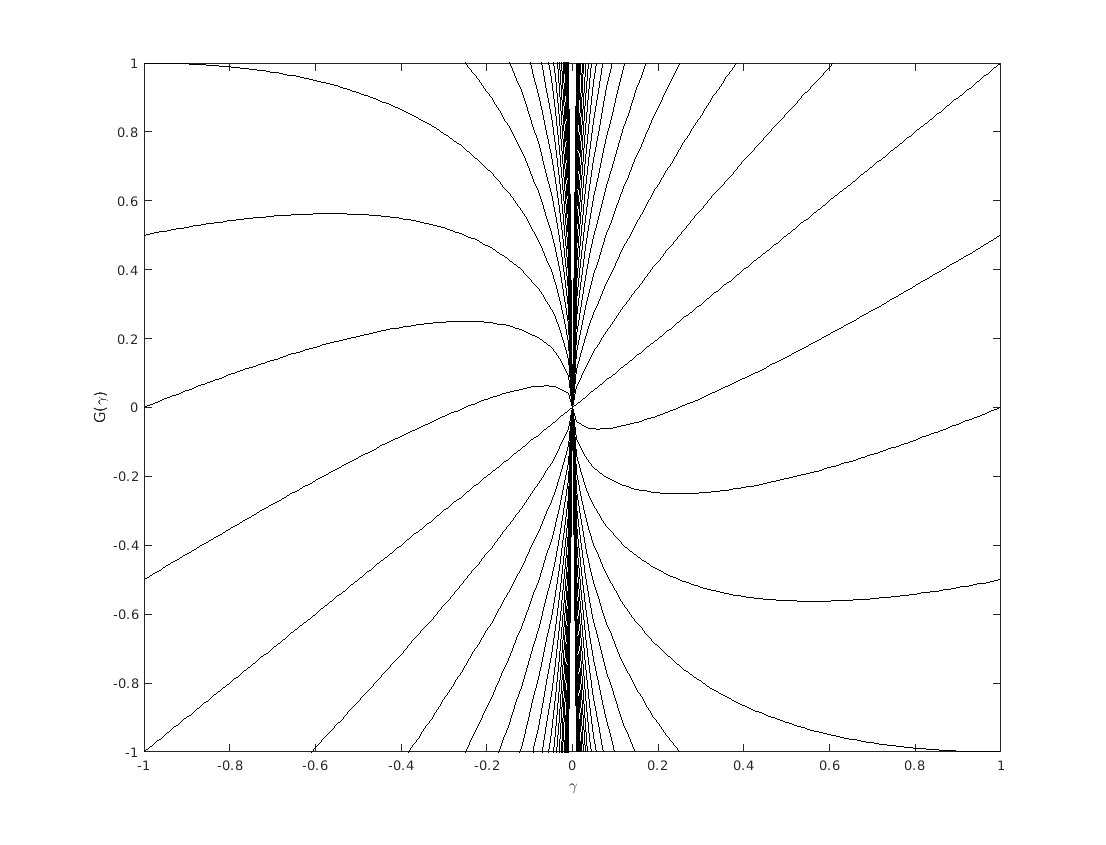
\includegraphics[width=0.7\textwidth]{clines.png}
\caption{The lines $g_C(x)$ which represent the geometry in which $g(x)$ is ideally monotonic.}
\label{fig:Clines}
\end{figure}

We begin by characterizing the four regions based on $x$ and $C$.
Firstly, if $C > 0$ then $g_C(x) > x$, and if $C<0$ then $g_C(x) < x$.
Region 1 is therefore where $C$ and $x-x^*$ have the same sign.
In this region $g_C'(x) > 1$, and so $g'(x) > 1$ or $C(x)$ will not be monotonic.

To describe region 2 we must find where $g_C(x)$ is less than the fixed point $x^*$:
\begin{align*}
&& x + C \sqrt{\abs{x - x^*}} & < x^* \\
&&                          C & < \frac{x^* - x}{\sqrt{\abs{x^*-x}}} \\
&&                            & < \sign(x^*-x) \sqrt{\abs{x^*-x}} \\
&&  			 \implies C^2 & \begin{cases} < \abs{x^*-x} & x^* > x \\ > \abs{x^*-x} & x^* < x . \end{cases}
\end{align*}
Region 2 is therefore where $\abs{x^*-x} > C^2$ and $x-x^*$ and $C$ have opposite signs.
The value of $g_C'(x)$ within region 2 is bounded:
\begin{align*}
g_C'(x) & = 1 + \sign(x-x^*) \frac{C}{2 \sqrt{\abs{x-x^*}}} \\
		& > 1 + \sign(x-x^*) \frac{C}{2 \abs{C}} \\
		& = 1 + \frac{1}{2} \sign(x-x^*) \sign(C) \\
		& = \frac{1}{2} , \\
g_C'(x) & < 1 + \sign(x-x^*) \lim_{x \rightarrow \pm \infty} \frac{C}{2 \sqrt{\abs{x-x^*}}} \\
		& = 1 + 0 = 1 , \\
\implies 1/2 < g_C'(x) & < 1 .
\end{align*}
Therefore, if $g(x)$ lies within region 2 and $g'(x) < 1/2$ then $C(x)$ is strictly monotonic and by extension Newton-Raphson converges.
Failing this, it is necessary that $g'(x) < 1$ for $C(x)$ to be monotonic.

For region 3 we ask where $g_C(x)$ is less than the line $2 x^* - x$:
\begin{align*}
x + C \sqrt{\abs{x-x^*}} & < 2 x^* - x \\
					C 	 & < \sign(x^*-x) 2 \sqrt{\abs{x^*-x}} \\
  \implies \frac{C^2}{4} & \begin{cases} < \abs{x^*-x} & x^* > x \\ > \abs{x^*-x} & x^* < x . \end{cases}
\end{align*}
Region 3 is therefore where $C^2/4 < \abs{x^*-x} < C^2$ and $x-x^*$ and $C$ have opposite signs.
Like region 2, the value of $g_C'(x)$ is bounded in region 3:
\begin{align*}
g_C'(x) & < \frac{1}{2} ,\\
g_C'(x) & > 1 + \sign(x-x^*) \frac{C}{\abs{C}} \\
		& = 0 , \\
\implies 0 < g_C'(x) & < 1/2 .
\end{align*}
Thus, if $g(x)$ lies within region 3 and $g'(x) < 0$ then Newton-Raphson converges.
For $C(x)$ to be monotonic it is necessary that $g'(x) < 1/2$.

Lastly, region 4 must then be where $\abs{x-x^*} < C^2/4$ and $x-x^*$ and $C$ have opposite signs.
As well, since $g_C''(x) \neq 0$ unless $C = 0$, $g_C'(x) < 0$ in region 4.
For $C(x)$ to be monotonic $g'(x)$ must likewise be negative.

\section{Application to alternating Schwarz}
\label{sec:appl}

Consider the alternating Schwarz method for a general second order nonlinear differential equation:
\begin{equation} \label{eq:AS}
\begin{cases} F(x,u_1^n,(u_1^n)',(u_1^n)'') = 0 & x \in [a,\beta] \\
u^n_1(a) = A \\
u^n_1(\beta) = u_2^{n-1}(\beta) \\
\end{cases}
\begin{cases} F(x,u^n_2,(u^n_2)',(u^n_2)'') = 0 & x \in [\alpha,b] \\
u^n_2(\alpha) = u^n_1(\alpha) \\
u^n_2(b) = B . \\
\end{cases}
\end{equation}
We can think of the operation to solve for $u_1^n$ as a function $G_1: \mathbb{R} \rightarrow \mathbb{R}$ such that $G_1(u_2^{n-1}(\beta)) = u_1^n(\alpha)$.
Likewise, $G_2(u_1^n(\alpha)) = u_2^n(\beta)$ and $G_2(G_1(\gamma)) = \gamma$ is a fixed point iteration.

Let $G(\gamma) = G_2 \circ G_1(\gamma)$, where $\gamma$ replaces $u^{n-1}_2(\beta)$ in equation (\ref{eq:AS}).
We will consider a single iteration and therefore drop the superscripts in the notation.
To establish how the solution of an ODE at a given point depends on the value of its endpoint, one can differentiate the ODE with respect to the endpoint:
\begin{align*}
\begin{cases} \pdxdy{F}{u} \dxdy{u_1}{\gamma} + \pdxdy{F}{u'} \dxdy{u_1'}{\gamma} + \pdxdy{F}{u''} \dxdy{u_1''}{\gamma} = 0 & x \in [a,\beta] \\
\dxdy{u_1(a)}{\gamma} = 0 \\
\dxdy{u_1(\beta)}{\gamma} = 1. \end{cases}
\end{align*}
Let $g_1(x) = \dxdy{u_1}{\gamma}$, then the ODE above may be written as:
\begin{equation*}
\begin{cases} J(u_1,u_1',u_1'') \cdot (g_1, g_1', g_1'') = 0 & x \in [a,\beta] \\ g_1(a) = 0 \\ g_1(\beta) = 1, \end{cases}
\end{equation*}
where $J(u,u',u'')$ is the Jacobian of $F(x,u,u',u'')$:
\begin{equation} \label{eq:Jacobian}
J(u,u',u'') = \left ( \pdxdy{F}{u}, \pdxdy{F}{u'}, \pdxdy{F}{u''} \right ) .
\end{equation}
Then $\dxdy{u_1(\alpha)}{\gamma} = g_1(\alpha)$.
Likewise, if $g_2(x) = \dxdy{u_2}{\gamma}$ then
\begin{equation*}
\begin{cases} J(u_2,u_2',u_2'') \cdot (g_2, g_2', g_2'') = 0 & x \in [\alpha,b] \\
g_2(\alpha) = \dxdy{u_1(\alpha)}{\gamma} = g_1(\alpha) \\ g_2(b) = 0 . \end{cases}
\end{equation*}
Therefore, $G'(\gamma) = G_2'(G_1(\gamma)) G_1'(\gamma) = g_2(\beta)$.
\begin{align*}
G'(\gamma) = \dxdy{u_2(\beta)}{\gamma} = \pdxdy{u_2(\beta)}{u_1(\alpha)} \dxdy{u_1(\alpha)}{\gamma} .
\end{align*}

There is an implicit assumption here that $G(\gamma)$ is differentiable.
If the problem is continuous with respect to the boundary data then $G(\gamma) \in C(\mathbb{R})$.
If, instead, a small perturbation in the boundary data leads to large change in the solution then we will lose the continuity of $G(\gamma)$ and most likely its differentiability.
One must then be careful when applying these methods to such problems.
Throughout this paper we will assume $G(\gamma) \in C(\mathbb{R})$.
We will also assume the problem is nonsingular and therefore the fixed point is unique.

Note if $F(x,u,u',u'')$ is linear in $u$, $u'$ and $u''$ then $u$ depends linearly on the boundary conditions.
This is reflected in $g_1$ and $g_2$ as neither depend on $\gamma$ so long as $J(u,u',u'')$ is not explicit in its inputs.
Thus, $G''(\gamma) = 0$ for linear problems and Newton-Raphson performed on $G(\gamma)$ converges in a single step.

Applying Newton's method to $G(\gamma)$ gives the following algorithm:
\begin{equation}
\begin{aligned} \label{alg:ASPN}
(1) & \begin{cases} F(x,u_1,u_1',u_1'') = 0 \\ u_1(a) = A \\ u_1(\beta) = \gamma_n \end{cases} &
(2) & \begin{cases} F(x,u_2,u_2',u_2'') = 0 \\ u_2(\alpha) = u_1(\alpha) \\ u_2(b) = B \end{cases} \\
(3) & \begin{cases} J(u_1,u_1',u_1'') \cdot (g_1,g_1',g_1'') = 0 \\ g_1(a) = 0 \\ g_1(\beta) = 1 \end{cases} &
(4) & \begin{cases} J(u_2,u_2',u_2'') \cdot (g_2,g_2',g_2'') = 0 \\ g_2(\alpha) = g_1(\alpha) \\ g_2(b) = 0 \end{cases} \\
(5) & \gamma_{n+1} = \gamma_n - \frac{ u_2(\beta) - \gamma_n }{g_2(\beta) - 1}. & &
\end{aligned}
\end{equation}
Steps $(2)$ and $(3)$ can be performed simultaneously.
Since step $(4)$ is a linear ODE it does not necessarily require step $(3)$ as one can solve instead
\begin{equation*}
(4*) \begin{cases} J(u_2,u_2',u_2'') \cdot (g_3,\textit{g}_3',\textit{g}_3'') = 0 \\
g_3(\alpha) = 1 \\ g_3(b) = 0 \end{cases}
\end{equation*}
and use $G'(\gamma) = g_1(\alpha) g_3(\beta)$ in place of $g_2(\beta)$ in step $(5)$.

We have examined in detail the desired properties of $G(\gamma)$ when solving a fixed point problem with Newton-Raphson (see section \ref{sec:nrfp}).
We focus on the necessary property that $G'(\gamma) \neq 1$.
The following theorem makes sure a reasonable $G(\gamma)$ satisfies this near $\gamma^*$.

\begin{thm}
Let $u(x)$ solve the second order ODE
\begin{equation*}
\begin{cases} F(u,u',u'') = 0 & x \in [a,b] \\ u(a) = A \\
u(b) = B . \end{cases}
\end{equation*}
Let $u_1(x)$, $u_2(x)$, $g_1(x)$, $g_2(x)$ be defined as in equation (\ref{alg:ASPN}) with $\gamma_n = \gamma$.
Let $G(\gamma) = u_2(\beta)$.
Let $J(x,y,z)$ be defined as in equation (\ref{eq:Jacobian}).

If $G(\gamma) \in C^1(\mathbb{R})$ and $J(u,u',u'')$ is nonsingular on both $[a,b]$ and $[\alpha,\beta]$, in the sense that the solution $v(x)$ to the ODE
\begin{equation*}
\begin{cases} J(u,u',u'') \cdot (v, v', v'') = 0 & x \in \Omega \\ v(x) = 0 & x \in \partial \Omega \end{cases}
\end{equation*}
is unique (and equal to the zero function),
then $G'(\gamma) \neq 1$ in an interval around $u(\beta)$.
As a corollary, the function $G(\gamma) - \gamma$ is monotonic in this interval.
\end{thm}

\begin{proof}
It suffices to show $G'(u(\beta)) \neq 1$.
As has been shown earlier, $G'(\gamma) = g_2(\beta)$.
Consider the difference between $g_1(x)$ and $g_2(x)$ in the region of overlap, $g(x) = g_2(x) - g_1(x)$.
This function satisfies:
\begin{equation*}
\begin{cases} J(u_2,u_2',u_2'') \cdot (g, g', g'') = \left ( J(u_2, u_2', u_2'') - J(u_1, u_1', u_1'') \right ) \cdot (g_1, g_1', g_1'') & x \in [\alpha, \beta] \\ g(\alpha) = 0 \\ g(\beta) = G'(\gamma) - 1. \end{cases}
\end{equation*}
For $\gamma = u(\beta)$, $u_1 = u_2 = u$ in the region of overlap and the right hand side is zero.
If $G'(u(\beta)) = 1$ then $g(x) = 0$ by the assumption that $J(u,u',u'')$ is nonsingular on $[\alpha,\beta]$.
Define the function $\hat{g}(x)$:
\begin{equation*}
\hat{g}(x) = \begin{cases} g_1(x) & x \in [a,\alpha] \\ g_2(x) & x \in (\alpha,b]. \end{cases}
\end{equation*}
This function satisfies:
\begin{equation*}
\begin{cases} J(u,u',u'') \cdot (\hat{g},\hat{g}',\hat{g}'') = 0 \\ \hat{g}(a) = \hat{g}(b) = 0. \end{cases}
\end{equation*}
By the assumption that $J(u,u',u'')$ is nonsingular on $[a,b]$ it must be that $\hat{g}(x) = 0$.
This contradicts $G'(u(\beta)) = 1$.
Therefore, $G'(u(\beta)) \neq 1$.
Since $G(\gamma) \in C^1(\mathbb{R})$ there is a neighbourhood of $u(\beta)$ for which $G'(\gamma) \neq 1$.
\end{proof}

If we consider instead $u_1 \neq u_2$ in the overlap region then the problem presented in the above theorem has a nonzero right hand side.
Because of this it is no longer necessary that $g(x) = 0$.
However, if $u_1$ and $u_2$ continue to converge to the same limit then the right hand side converges to zero.
The function $g(x)$ then has a magnitude related to the difference between $u_1$ and $u_2$.
%include lemma on relation, especially if J(u,u',u'') is Lipschitz

One can use similar strategies to prove that $G(\gamma)$ is monotonic under certain conditions.
For $\alpha$ in some neighbourhood of $\beta$ this implies $G'(\gamma)>0$, as an increasing boundary condition should cause the solution nearby to likewise increase.
The theorem presents this exclusively for Dirichlet transmission conditions, but the theorem applies more broadly.

\begin{thm} \label{thm:mono}
If the problem
\begin{equation*}
\begin{cases} F(u,u',u'') = 0 & x \in \Omega \\ u(x) = h(x) & x \in \partial \Omega \end{cases}
\end{equation*}
is nonsingular on $[a,\alpha]$ and $[\beta,b]$, in the sense that there exists a unique solution to the problem on those domains and that the continuations of these solutions are also unique, then the function $G(\gamma)$ is strictly monotonic.
\end{thm}

\begin{proof}
It suffices to show that $G(\gamma_1) = G(\gamma_2)$ implies $\gamma_1 = \gamma_2$.

Let $u^j_1$ solve the problem on $[a,\beta]$ with $u^j_1(\beta) = \gamma_j$.
Likewise, $u^j_2$ solves the problem on $[\alpha, b]$ with $u^j_2(\alpha) = u^j_1(\alpha)$.
Suppose $u^1_2(\beta) = u^2_2(\beta)$.
Then both $u^1_2$ and $u^2_2$ solve the same problem on $[\beta,b]$.
By assumption, this must mean $u^1_2 = u^2_2$ and $u^1_1(\alpha) = u^2_1(\alpha)$.
By a similar argument, this implies $u^1_1$ and $u^2_1$ solve the same problem on $[a,\alpha]$.
Again by assumption $u^1_1 = u^2_1$ and $\gamma_1 = \gamma_2$.
\end{proof}

While we are now confident that many of the problems we encounter will have $G'(\gamma) \neq 0$ we are more interested in if $G(\gamma) - \gamma$ is monotonic.
To that end, we present the following lemma, which acts as a converse to the mean value theorem for certain functions, and a corollary to this lemma giving sufficient conditions for $G'(\gamma) \neq 1$.

\begin{lemma}
If $f \in C^2([a,b])$, $f''(x) \neq 0$ for all $x \in (a,b)$ and $f'(c) = 0$ for some $c \in (a,b)$ then there exists $x_0 \in (a,b)$ such that $f(x_0)$ is equal to either $f(a)$ or $f(b)$.
Moreover, there is only one local extrema on this interval.
\end{lemma}

\begin{proof}
We begin by showing that if $f'(c_1) = f'(c_2) = 0$ then $c_1 = c_2$.
Consider the region $[c_1,c_2]$.
By the mean value theorem there must exist a point $c_3 \in (c_1,c_2)$ such that $f''(c_3) = 0$.
This contradicts the assumption that $f''(x) \neq 0$ for all $x \in (a,b)$, unless $(c_1,c_2)$ is the empty set.
Therefore, $c_1 = c_2$.

Suppose the statement is not true, that is for all $x_0 \in (a,b)$ $f(x_0) \neq f(a)$ and $f(x_0) \neq f(b)$.
Then it must be that either $f(a) < f(x_0) < f(b)$ for all $x_0 \in (a,b)$ or $f(a) > f(x_0) > f(b)$.
Then $f(x)$ is monotonic on $[a,c_1]$ and $[c_2,b]$ where $f'(c_1) = f'(c_2) = 0$.
We have already shown that $c_1 = c_2 = c$.
Thus $f(x)$ is monotonic on $[a,b]$, and $f'(x) \geq 0$ or $f'(x) \leq 0$.
WLOG we consider the former.

Let $S_1 = [a,c)$ and $S_2 = (c,b]$, and let $s_1 = \max_{x \in S_1} f'(x) > 0$ and $s_2 = \max_{x \in S_2} f'(x)) > 0$.
WLOG, $s_1 > s_2$.
Since $f'(x)$ is continuous, there exists $x_1 \in S_1$ such that $f'(x_1) = s_2 = f'(x_2)$ for some $x_2 \in S_2$.
Therefore, again by the mean value theorem, $f''(x_3) = 0$ for some $x_3 \in (x_1,x_2)$.
This contradicts the assumption that $f''(x) \neq 0$ on the interval.
Thus, it must be that the statement is true.
\end{proof}

\begin{cor}
If $G(\gamma) \in C^2(\mathbb{R})$ and $G''(\gamma^*) = 0$ implies $G(\gamma^*) = \gamma^*$ then either $G'(\gamma) \neq 1$ for all $\gamma$ or the problem is singular.
\end{cor}

\begin{proof}
Consider $f(\gamma) = G(\gamma) - \gamma$ and the domains $(-\infty,\gamma^*]$ and $[\gamma^*,\infty)$.
Apply the previous lemma to $f(\gamma)$, noting that $f(\gamma^*) = 0$ and $\liminfty{\pm \gamma} f(\gamma) = \pm \infty$.
Therefore, if $f'(\gamma_1) = 0$ for some $\gamma_1 \neq \gamma^*$ then $f(\gamma_2) = 0$ for some $\gamma_2 \neq \gamma^*$.
This implies $G(\gamma)$ has two fixed points, and therefore the problem has two solutions.
\end{proof}

We examine the problem
\begin{equation*}
\begin{cases} u_{xx} = 0 & x \in [a,b] \\ u(a) = u(b) = 0 \end{cases}
\end{equation*}
with exact solution $u=0$ and Robin transmission conditions:
\begin{equation*}
u'^n_1(\beta) + C_1 u^n_1(\beta) = \gamma, \quad u'^n_2(\alpha) + C_2 u^n_2(\alpha) = u'^n_1(\alpha) + C_2 u^n_1(\alpha) .
\end{equation*}
The solutions at each step are linear functions, and so the fixed point function $G(\gamma)$ is straighforward to find:
\begin{equation*}
G(\gamma) = \gamma \frac{1 - C_1(b-\beta)}{1 + C_1(\beta-a)} \frac{1 + C_2(\alpha-a)}{1 - C_2(b - \alpha)} .
\end{equation*}

Since $G(\gamma)$ is linear, the Newton-Raphson iteration converges in a single iteration.
More interestingly, the slope $G'(\gamma)$ may take on any real value depending on the choices of $C_1$ and $C_2$.
Fixing $\alpha$ and $\beta$ and considering $G'(\gamma)$ as a function on $\mathbb{R}^2$, we have that $G':\mathbb{R}^2 \rightarrow \mathbb{R}$.

Such a function is not continuous: there are singularities along the lines $C_1 = \frac{-1}{\beta-a}$ and $C_2 = \frac{1}{b-\alpha}$.
There are also roots along the lines $C_1 = \frac{1}{b-\beta}$ and $C_2 = \frac{-1}{\alpha-a}$.
These lines also divide the boundaries between which of the four regions the fixed point iteration lies within.
While near the singularities, $G(\gamma)$ is in either region 1 or 4; while away, regions 2 or 3.
When one of the two constants is between these lines while the other is not, $G(\gamma)$ is in either region 3 or 4; if both or neither are between the lines then $G(\gamma)$ is in region 1 or 2.

\begin{figure}
\centering
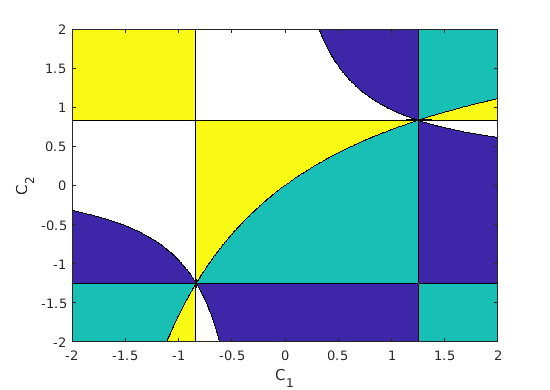
\includegraphics[width=0.7\textwidth]{exp9_01.png}
\caption{$G'(\gamma)$ as a function of $C_1$ and $C_2$ for $a = -b = -1$ and $\alpha = -\beta = -0.2$.
The regions yellow, green, blue and white correspond to the regions 1, 2, 3 and 4, respectively.}
\end{figure}

While this only applies to this particular problem, it shows that the fixed point iteration $G(\gamma)$ may appear in any of the four regions with any slope.

Consider a second example for which we may write out explicitly $G'(\gamma^*)$:
\begin{equation*}
\begin{cases} u_{xx} - C \sin(u) = 0 & x \in [-1,1] \\ u(-1) = u(1) = 0 \end{cases}
\end{equation*}
with $\alpha = -\beta = -0.2$ and $C>0$.
The solution to the problem is $u=0$.
Using the same Robin transmission conditions as earlier, we have the following equation for $G'(\gamma^*)$:
\begin{equation*}
G'(\gamma^*) = \frac{\sqrt{C} \cosh(0.8 \sqrt{C}) + C_2 \sinh (0.8 \sqrt{C})}{\sqrt{C} \cosh(1.2 \sqrt{C}) + C_1 \sinh(1.2 \sqrt{C})} \frac{\sqrt{C} \cosh((-0.8) \sqrt{C}) + C_1 \sinh ((-0.8) \sqrt{C})}{\sqrt{C} \cosh((-1.2) \sqrt{C}) + C_2 \sinh((-1.2) \sqrt{C})} .
\end{equation*}

\begin{figure}
\centering
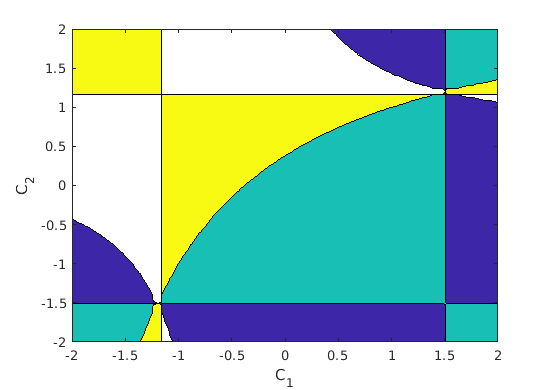
\includegraphics[width=0.7\textwidth]{exp12_01.png}
\caption{$G'(\gamma^*)$ as a function of $C_1$ and $C_2$ for the second example problem with $C=1$.
The regions yellow, green, blue and white correspond to the regions 1, 2, 3 and 4, respectively.}
\end{figure}

The regions that $G(\gamma)$ lies in are determined by the value of $G'(\gamma^*)$ and certain conditions.
For example, if the problem is nonsingular then $G(\gamma)$ cannot cross between regions 1 and 2.
If $G(\gamma)$ is known to be monotonic then it cannot cross between regions 2 and 3.
The example problem presented here is known to be nonsingular and the corresponding $G(\gamma)$ is monotonic for all $C_1$ and $C_2$ (nb: prove?), and so $G'(\gamma^*)$ informs us whether the fixed point iteration lies within regions 1, 2 or the combination of 3 and 4 for every choice of $\gamma$.

\begin{figure}
\centering
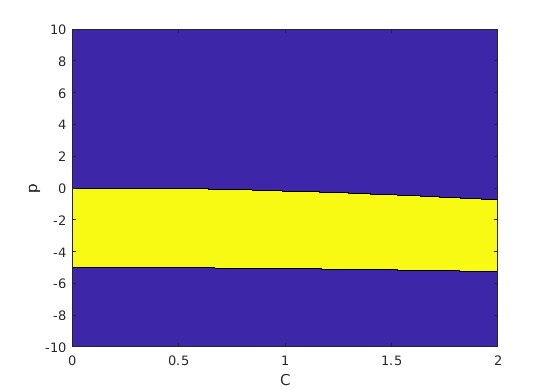
\includegraphics[width=0.7\textwidth]{exp12_02.png}
\caption{$G'(\gamma^*)$ as a function of $p = C_1 = -C_2$ and $C$.
The region blue corresponds to region 2 and the region yellow to region 3.}
\end{figure}

For $C=1$ and $p = C_1 = -C_2 = -2$ we have that $G(\gamma)$ is in region 1.
As such, the fixed point iteration diverges away from the root.
The Newton-Raphson iteration, on the other hand, will converge.
This may be seen in figure \ref{fig:exCsin3}.
The choice $p>0$ is apparently natural and for most problems examined will place $G(\gamma)$ in region 2.

\begin{figure}
\centering
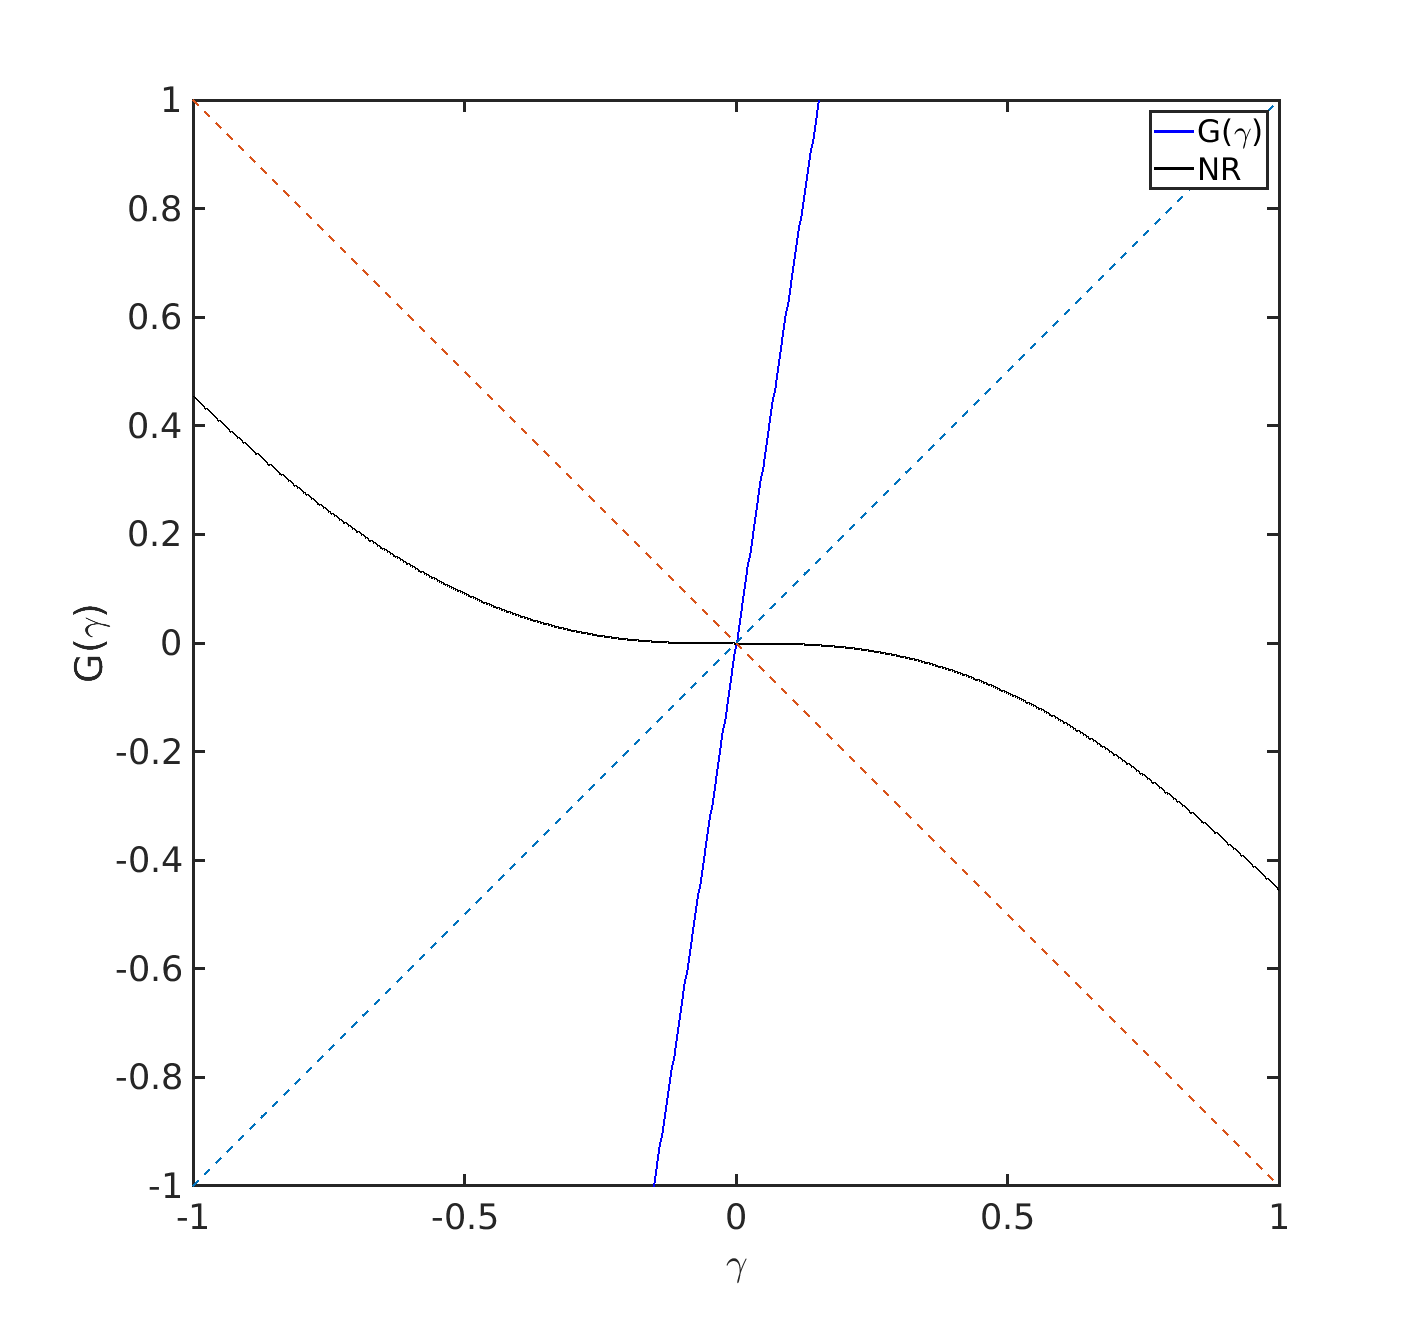
\includegraphics[width=0.7\textwidth]{exp12_03.png}
\caption{The fixed point function $G(\gamma)$ and the corresponding Newton-Raphson iteration for the second example problem with $C=1$ and $p=C_1 = -C_2 = -2$.}
\label{fig:exCsin3}
\end{figure}

For $C<0$ the problem in $u$ is possibly singular, especially with Robin boundary conditions and certain subintervals.

Under certain conditions one may be able to show that $G(\gamma)$ is restricted to specific regions.
As an example, we reprove a result from Lui \cite{lui1999schwarz}.

\begin{thm}[Theorem 2 from \cite{lui1999schwarz}] \label{thm:lui}
Consider the equation
\begin{equation*}
\begin{cases} u''(x) + f(x,u,u') = 0 & x \in [a,b] \\ u(a) = u(b) = 0 \end{cases}
\end{equation*}
under the assumptions that
\begin{itemize}
\item $f \in C^1 \left ( [a,b] \times \mathbb{R} \times \mathbb{R} \right )$ ,
\item $\pdxdy{f(x,v,v')}{u} \leq 0$ for all $x \in [a,b]$ and $v \in H_0^1([a,b])$ ,
\item $\abs{f(x,v,v')} \leq C(1 + \abs{v'}^\eta)$ for all $x \in [a,b]$ and $v \in H_0^1([a,b])$ and some $C > 0$, $0 < \eta < 1$ .
\end{itemize}
The problem is solved using alternating Schwarz with two subdomains and Dirichlet transmission conditions.
Then $G(\gamma)$ for this problem lies within region 2.
\end{thm}

\begin{proof}
It suffices to prove that the problem is nonsingular and $0 < G'(\gamma) < 1$ for all $\gamma \in \mathbb{R}$.
The nonsingularity of the problem is guaranteed by proposition 2 from \cite{lui1999schwarz}.
As Lui points out, this also means the problem is nonsingular on any subdomain.
Using theorem \ref{thm:mono} this gives monotonicity of $G(\gamma)$.
Moreover, if $u(x)=0$ for any $x \in (a,b)$ then the problem would be singular on the domains $[a,x]$ and $[x,b]$.
As such, $u(x)$ has the same sign as $\gamma$ and $G'(\gamma) > 0$.

Consider the problem in $g_1$:
\begin{equation*}
\begin{cases} g_1''(x) + \pdxdy{f}{u} g_1 + \pdxdy{f}{u'} g_1' = 0 & x \in [a,\beta] \\ g_1(a) = 0 \\ g_1(\beta) = 1 . \end{cases}
\end{equation*}
From the second assumption on $f$ the operator on $g_1$ satisfies a maximum principle (see, for example, \cite{lui1999schwarz}).
Therefore, $g_1(x) < 1$ for all $x \in (a,\beta)$.
By the same reasoning, $g_2(x) < g_1(\alpha) < 1$ for all $x \in (\alpha, b)$ and $G'(\gamma) < 1$.
Incidentally, the same maximum principle applies for the operator on $-g_1$ and $-g_2$, and so $G'(\gamma) > 0$ as we had before.
\end{proof}

Recall from section \ref{sec:nrfp} the function $C(x)$.
In the context of domain decomposition, this function becomes:
\begin{equation*}
C(\gamma) = \frac{ G(\gamma) - \gamma}{\sqrt{\abs{\gamma - \gamma^*}}} .
\end{equation*}
While it is ideal that this function is strictly monotonic, this cannot be guaranteed.

\section{Period doubling in RASPEN (or RASPEN-like methods)}

Take as a counterexample the following differential equation:
\begin{equation*}
u''(x) - \sin(3.6 u(x)) = 0 .
\end{equation*}
With homogeneous Dirichlet boundary conditions the solution to this problem is the zero function.
Using Dirichlet transmission conditions one arrives at the function $G(\gamma)$ depicted in figure \ref{fig:exsin}.

\begin{figure}
%	\begin{subfigure}{0.5\textwidth}
%		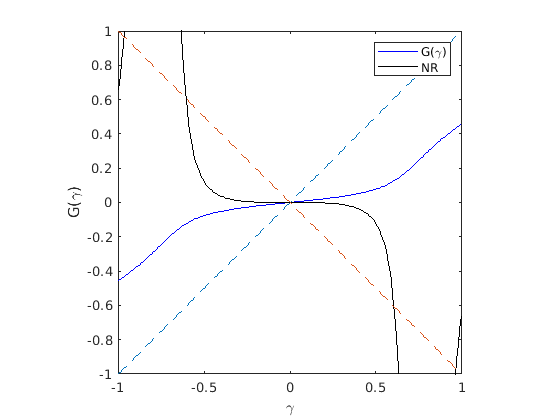
\includegraphics[width=\textwidth]{ExSin01.png}
%	\end{subfigure}
%	\begin{subfigure}{0.5\textwidth}
%		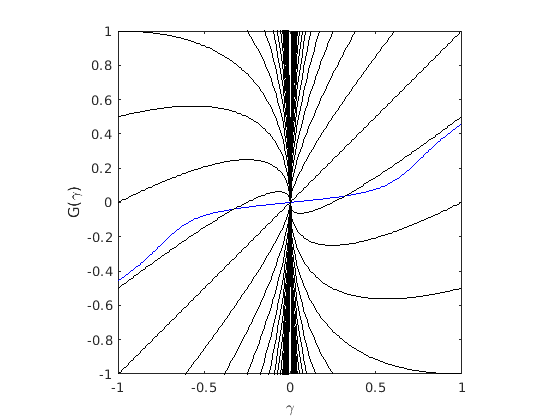
\includegraphics[width=\textwidth]{ExSin02.png}
%	\end{subfigure}
	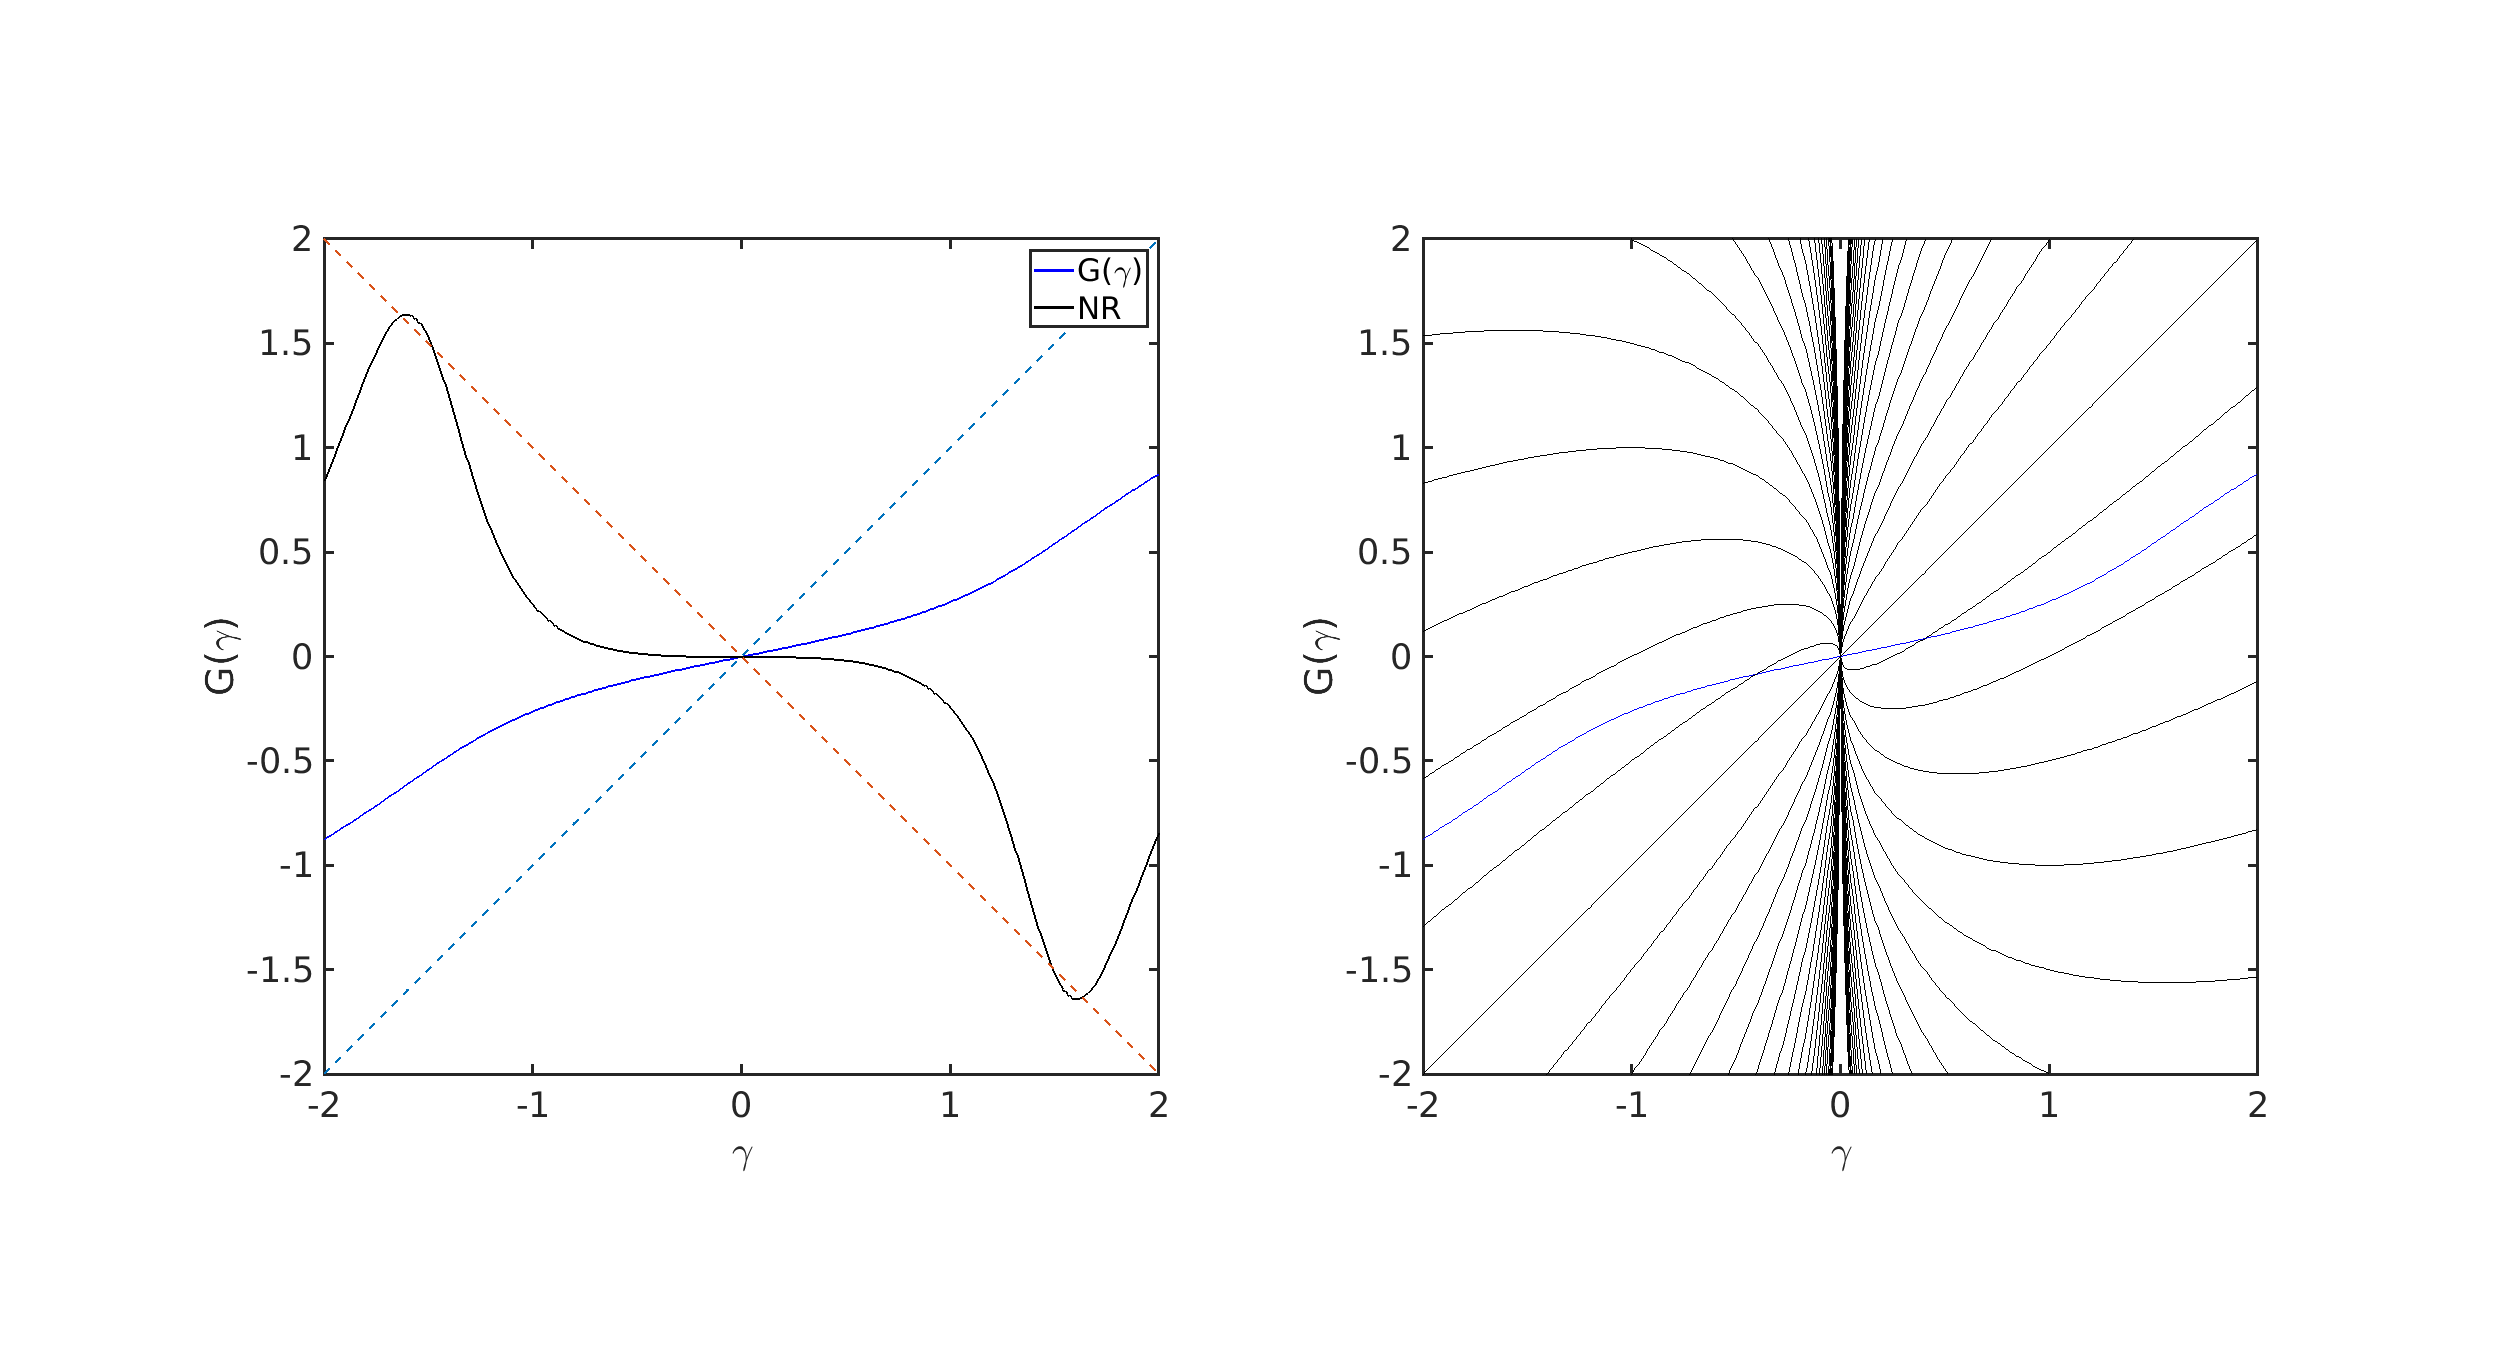
\includegraphics[width=\textwidth]{exp9_02.png}
	\caption{The function $G(\gamma)$.
	On the left, the corresponding Newton-Raphson iteration is plotted along with the lines $y=\gamma$ and $y=2 \gamma^* - \gamma$.
	On the right, the lines $g_C(\gamma)$ show the function $C(\gamma)$ is not monotonic for this problem.}
	\label{fig:exsin}
\end{figure}

As seen in the figure, where $G(\gamma)$ is not monotonic with respect to the geometry of the lines $g_C(\gamma)$ (equivalent to $C(\gamma)$ no longer monotonic) the Newton-Raphson iteration enters into region 4.
Due to the symmetry of the function $G(\gamma)$, this creates at least two 2-cycles where $G(\gamma)$ meets the line $y = 2 \gamma^* - \gamma$.
One of these 2-cycles is stable, and taking $\gamma_0 = 1.6$ (or somewhere nearby) the Newton-Raphson preconditioning will cause the iterations to converge to this cycle.

Indeed, the differential equation
\begin{equation} \label{eq:sin}
u''(x) - \sin \left ( a u(x) \right ) = 0
\end{equation}
admits a period doubling set of cycles in the parameter $a$ for the domain $[-1,1]$, $\alpha = -\beta = -0.2$ and $\gamma_0 = \pm 1.6$.
The bifurcation diagram is shown in figure \ref{fig:bifurc}.
The red points displayed result from choosing $\gamma_0 = -1.6$, while the black points from choosing $\gamma_0 = 1.6$.
The first bifurcation is the separation of the 2-cycle into two separate 2-cycles instead of the usual 4-cycle.
Once this is done, period doubling sets in for each of these 2-cycles until the onset of chaos.

The chaos of this system collapses once it spreads out sufficiently to include the region where Newton-Raphson is convergent.
That is, when the slope moves close enough to 1 the range of the cycles is so wide that it intersects with areas near enough to the fixed point such that Newton-Raphson converges quadratically.
This collapse occurs between $a = 3.812$ and $a=3.813$, after which these values of $\gamma_0$ (and possibly all values) lead to quadratically convergent sequences.

\begin{figure}
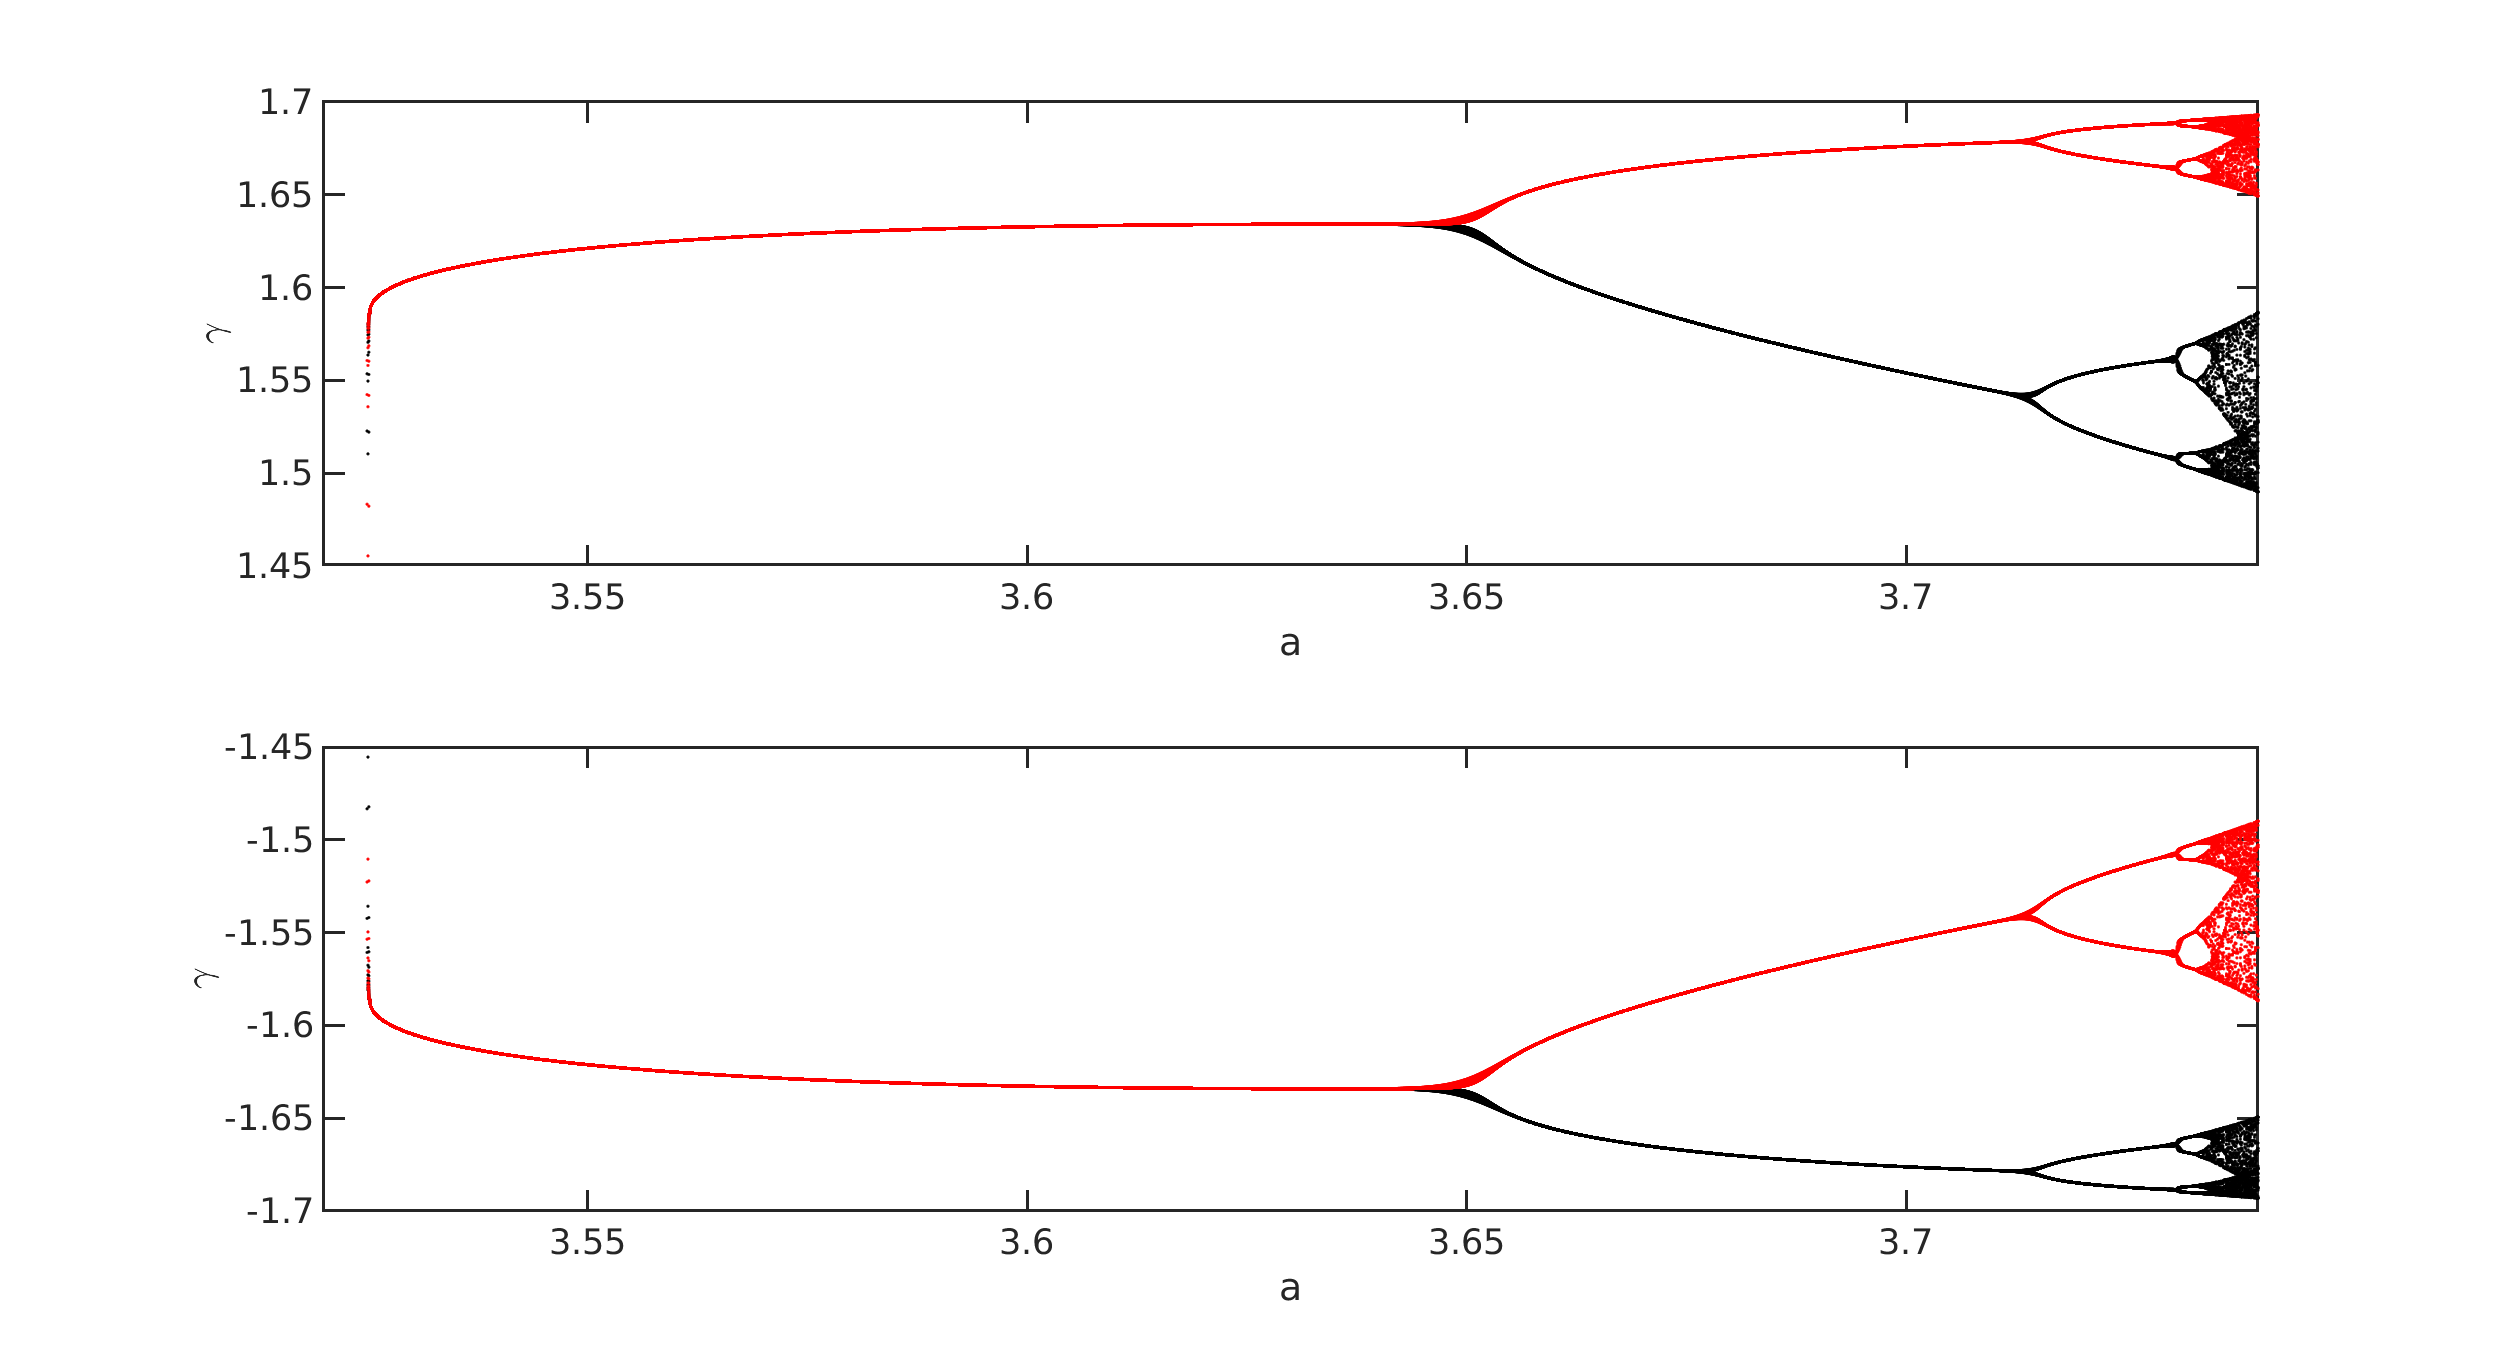
\includegraphics[width=\textwidth]{bifurcation_all.png}
\caption{The bifurcation diagram for the sinusoid counterexample in the parameter $a$.
The first bifurcation point is the separation of the 2-cycle into two separate 2-cycles, rather than one 4-cycle.
After this, the bifurcation proceeds normally.}
\label{fig:bifurc}
\end{figure}

\subsection{Wellposedness}

\begin{lemma}[Wellposedness]
Equation \ref{eq:sin} with homogeneous boundary conditions on the domain $[-1,1]$ is well-posed for $u \in C^2[-1,1]$ and real-valued.
\end{lemma}

\begin{proof}
Firstly we prove that any solution $u(x)$ to the equation lies between $1$ and $-1$.
First note that $\abs{u''(x)} \leq 1$ since $u''(x) = \sin(au(x))$.
Suppose there is a point $\hat{x}$ such that $u(\hat{x}) = 1$.
Then by the mean value theorem there exist $c_1 \in [-1,\hat{x})$ and $c_2 \in (\hat{x}, 1]$ such that
$u'(c_1) = 1 / (\hat{x} + 1)$
and
$u'(c_2) = -1 / (1 - \hat{x})$.
By the same theorem there exists $c_3 \in (c_1,c_2)$ such that
$u''(c_3) = (u'(c_2) - u'(c_1)) / (c_2 - c_1)$.
That is
\begin{align*}
u''(c_3) & = \frac{ -\frac{1}{1 - \hat{x}} - \frac{1}{\hat{x}+1} }{c_2 - c_1}
		  = \frac{ -\frac{ \hat{x} - 1 + \hat{x} - 1}{(1+\hat{x})(1-\hat{x})} }{c_2 - c_1}
		  = \frac{ \frac{-2}{1 - \hat{x}^2} }{c_2 - c_1} \\
		 & \leq \frac{ \frac{-2}{1 - \hat{x}^2} }{2} = \frac{-1}{1 - \hat{x}^2} \leq -1
\end{align*}
which contradicts $\abs{u''(x)} \leq 1$ and so $u(x) < 1$.
Similarly, $u(x) > -1$.

Secondly we prove that $u(x) = 0$ is the only solution lying between $1$ and $-1$.
Since the value of $u(x)$ is less than one in magnitude for all values of $x \in [-1,1]$ we may write
\begin{equation*}
u(x) = \epsilon u_1(x) + \epsilon^2 u_2(x) + \epsilon^3 u_3(x) + \dots
\end{equation*}
for some $0 < \epsilon < 1$ such that $-1 \leq u_i(x) \leq 1$ for all $x \in [-1,1]$.
Then one may expand $\sin(au(x))$ into a Taylor series:
\begin{align*}
\sin(au(x)) & = au(x) - a^3 u^3(x) / 6 + \dots \\
			& = \epsilon a u_1(x) + \epsilon^2 a u_2(x) + \epsilon^3 a u_3(x) - \epsilon^3 a^3 u_1^3(x)/6 + \dots
\end{align*}
The equation in $\order{\epsilon}$ is:
\begin{equation*}
u_1''(x) - au_1(x) = 0
\end{equation*}
which, combined with the homogeneous boundary conditions, has the unique solution $u_1(x) = 0$.
The same is true of $u_2(x)$ in solving the equation in $\order{\epsilon^2}$.
For $\order{\epsilon^3}$, given that $u_1(x) = 0$ we have the same equation for $u_3(x)$, so that $u_3(x) = 0$ as well.
One may continue this for all orders of $\epsilon$.
Therefore, $u(x) = 0$.
% does the presence of $a$ change the result?
\end{proof}

\subsection{Changing overlap}

The overlap affects the position and length of the interval in $a$ where the bifurcation occurs.
For $\alpha = -\beta = -0.1$, the interval is roughly $[2.25,2.4]$ with $\gamma_0 = \pm 2$.
For $\alpha = -\beta = -0.4$, the interval is roughly $[9.10,9.155]$ with $\gamma_0 = \pm 1.45$.

The bifurcation becomes smaller the larger the overlap, as may be seen when comparing figures \ref{fig:overlap1} and \ref{fig:overlap2}.
Note that we may not have chosen $\gamma_0$ such that we land within a cycle for all values of $a$, $\alpha$ and $\beta$.
As such, the exact length of each bifurcation diagram here is only an estimate, though the distance between each bifurcation should be indicative of their sizes.

For exampe, for $\alpha = -\beta = -0.1$ we estimate the distance between the 4-cycle and the 8-cycle as approximately 0.03.
For $\alpha = -\beta = -0.2$ this value is roughly 0.07 and for $\alpha = -\beta = -0.4$ it is roughly 0.018.
The dependence of these distances on the size of the overlap is then nonlinear.

\begin{figure}
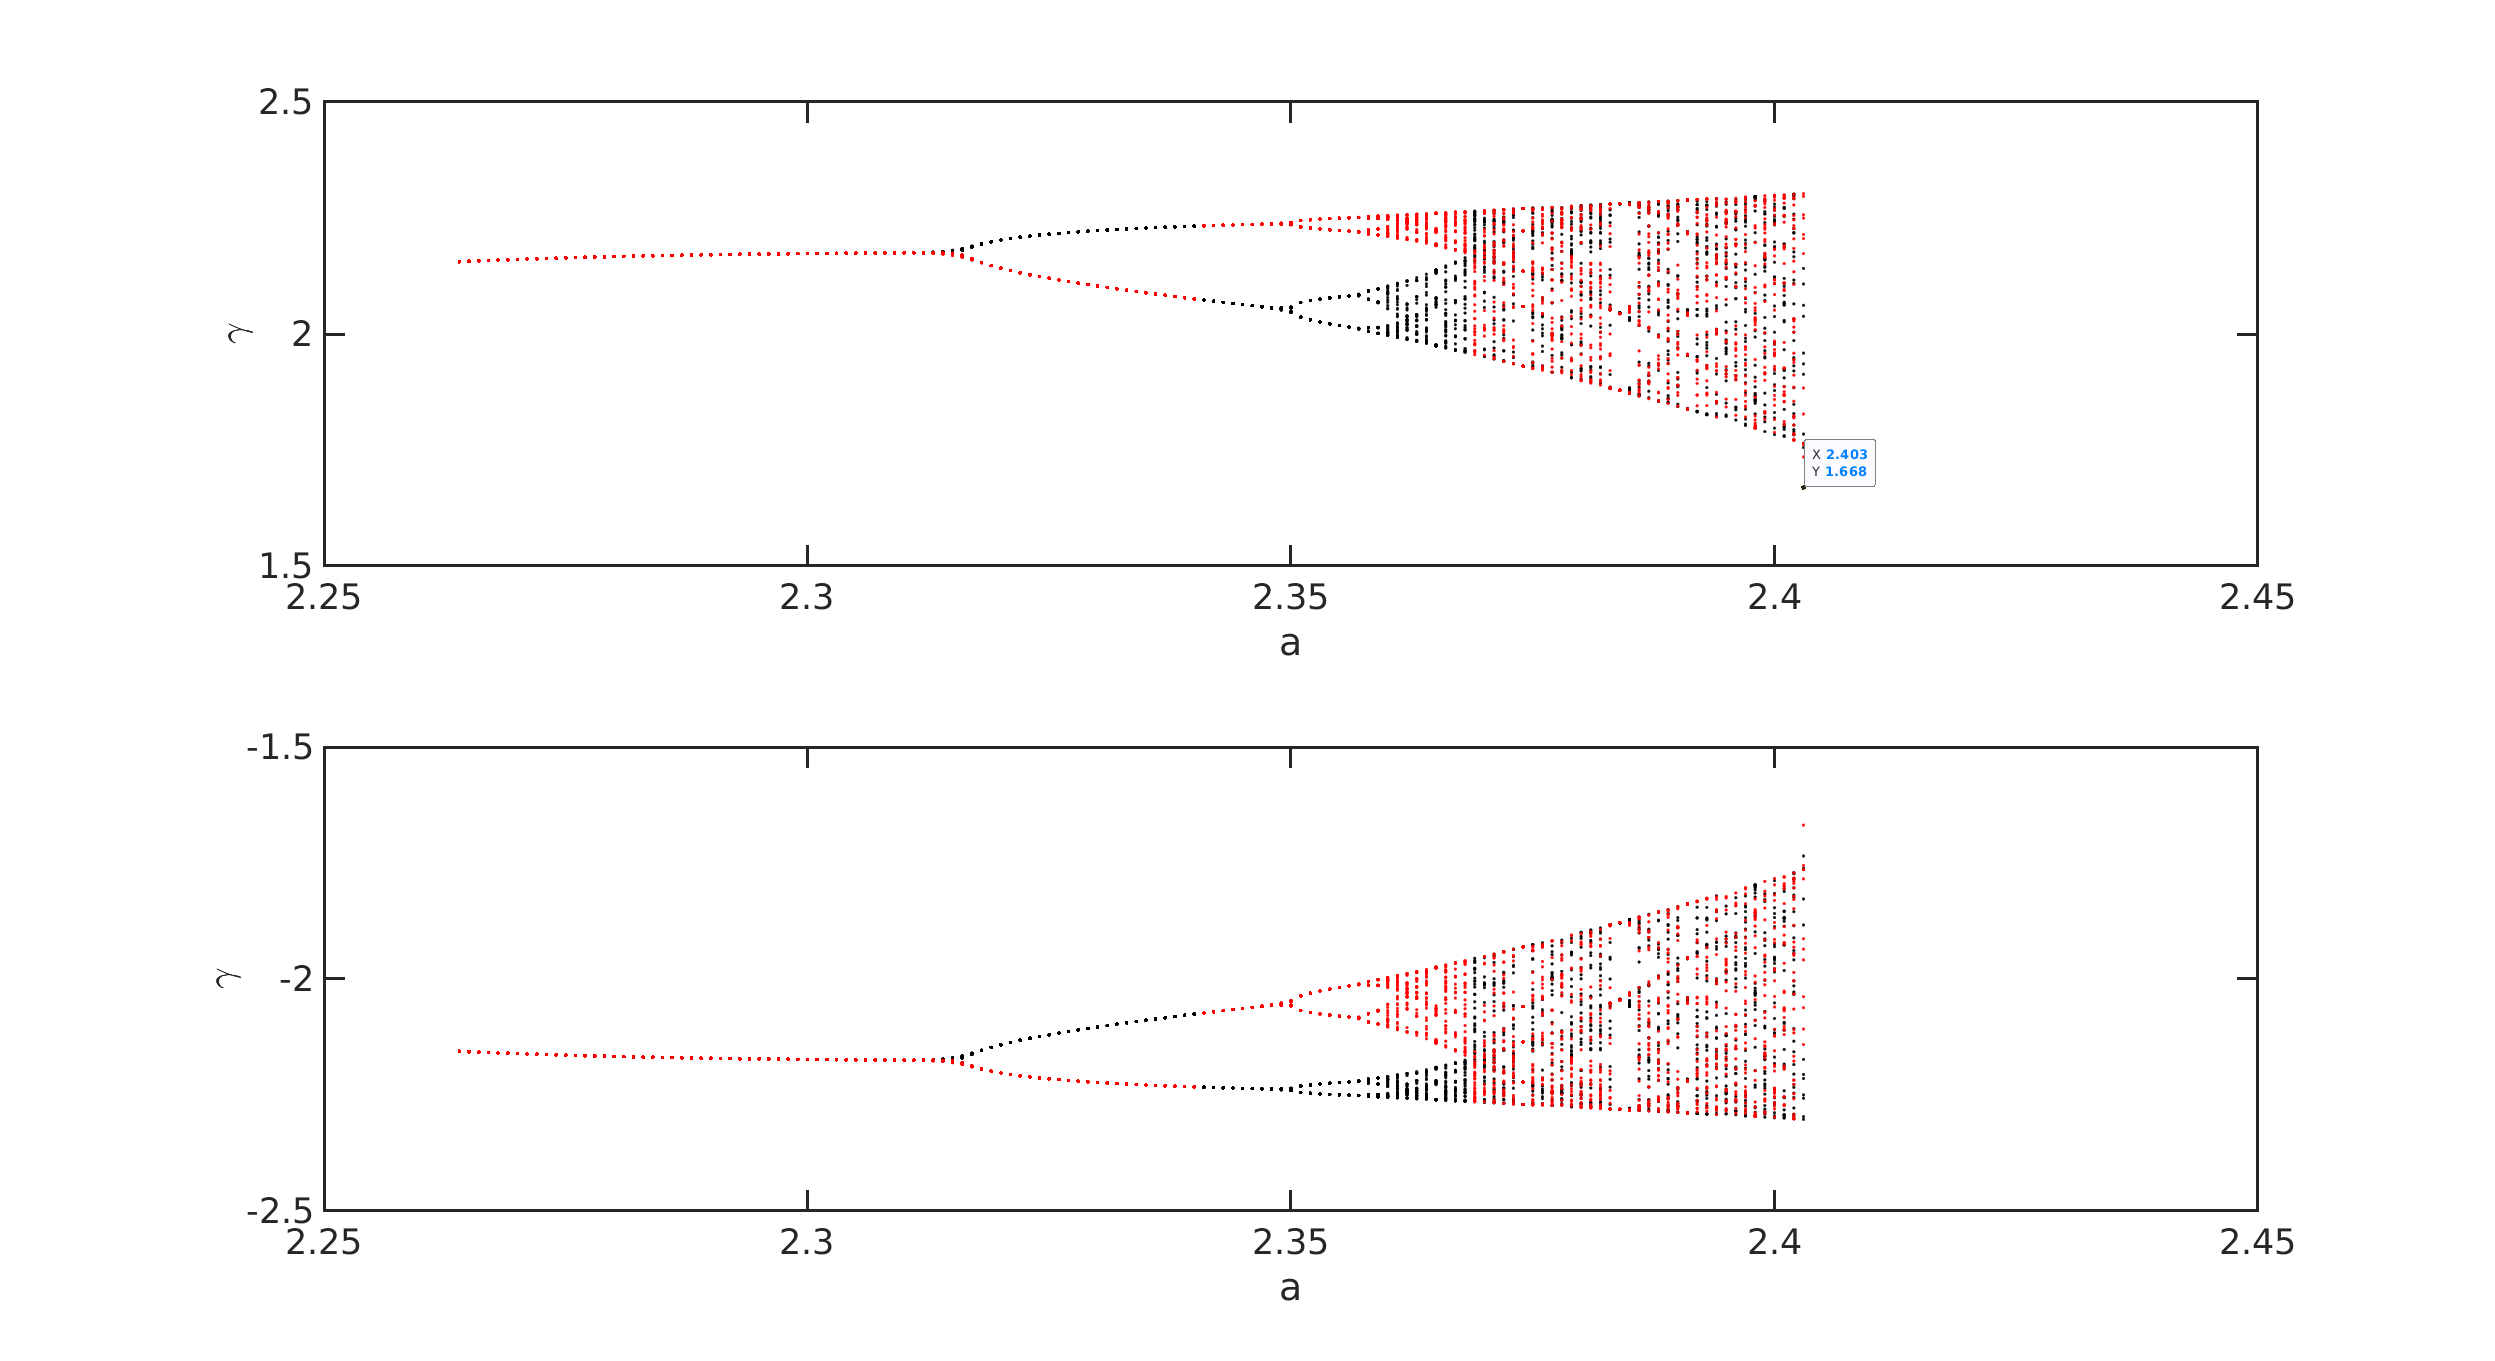
\includegraphics[width=\textwidth]{bifurcation_overlap1.png}
\caption{Bifurcation diagram with $\alpha = -\beta = -0.1$ and $\gamma_0 = \pm 2$.}
\label{fig:overlap1}
\end{figure}

\begin{figure}
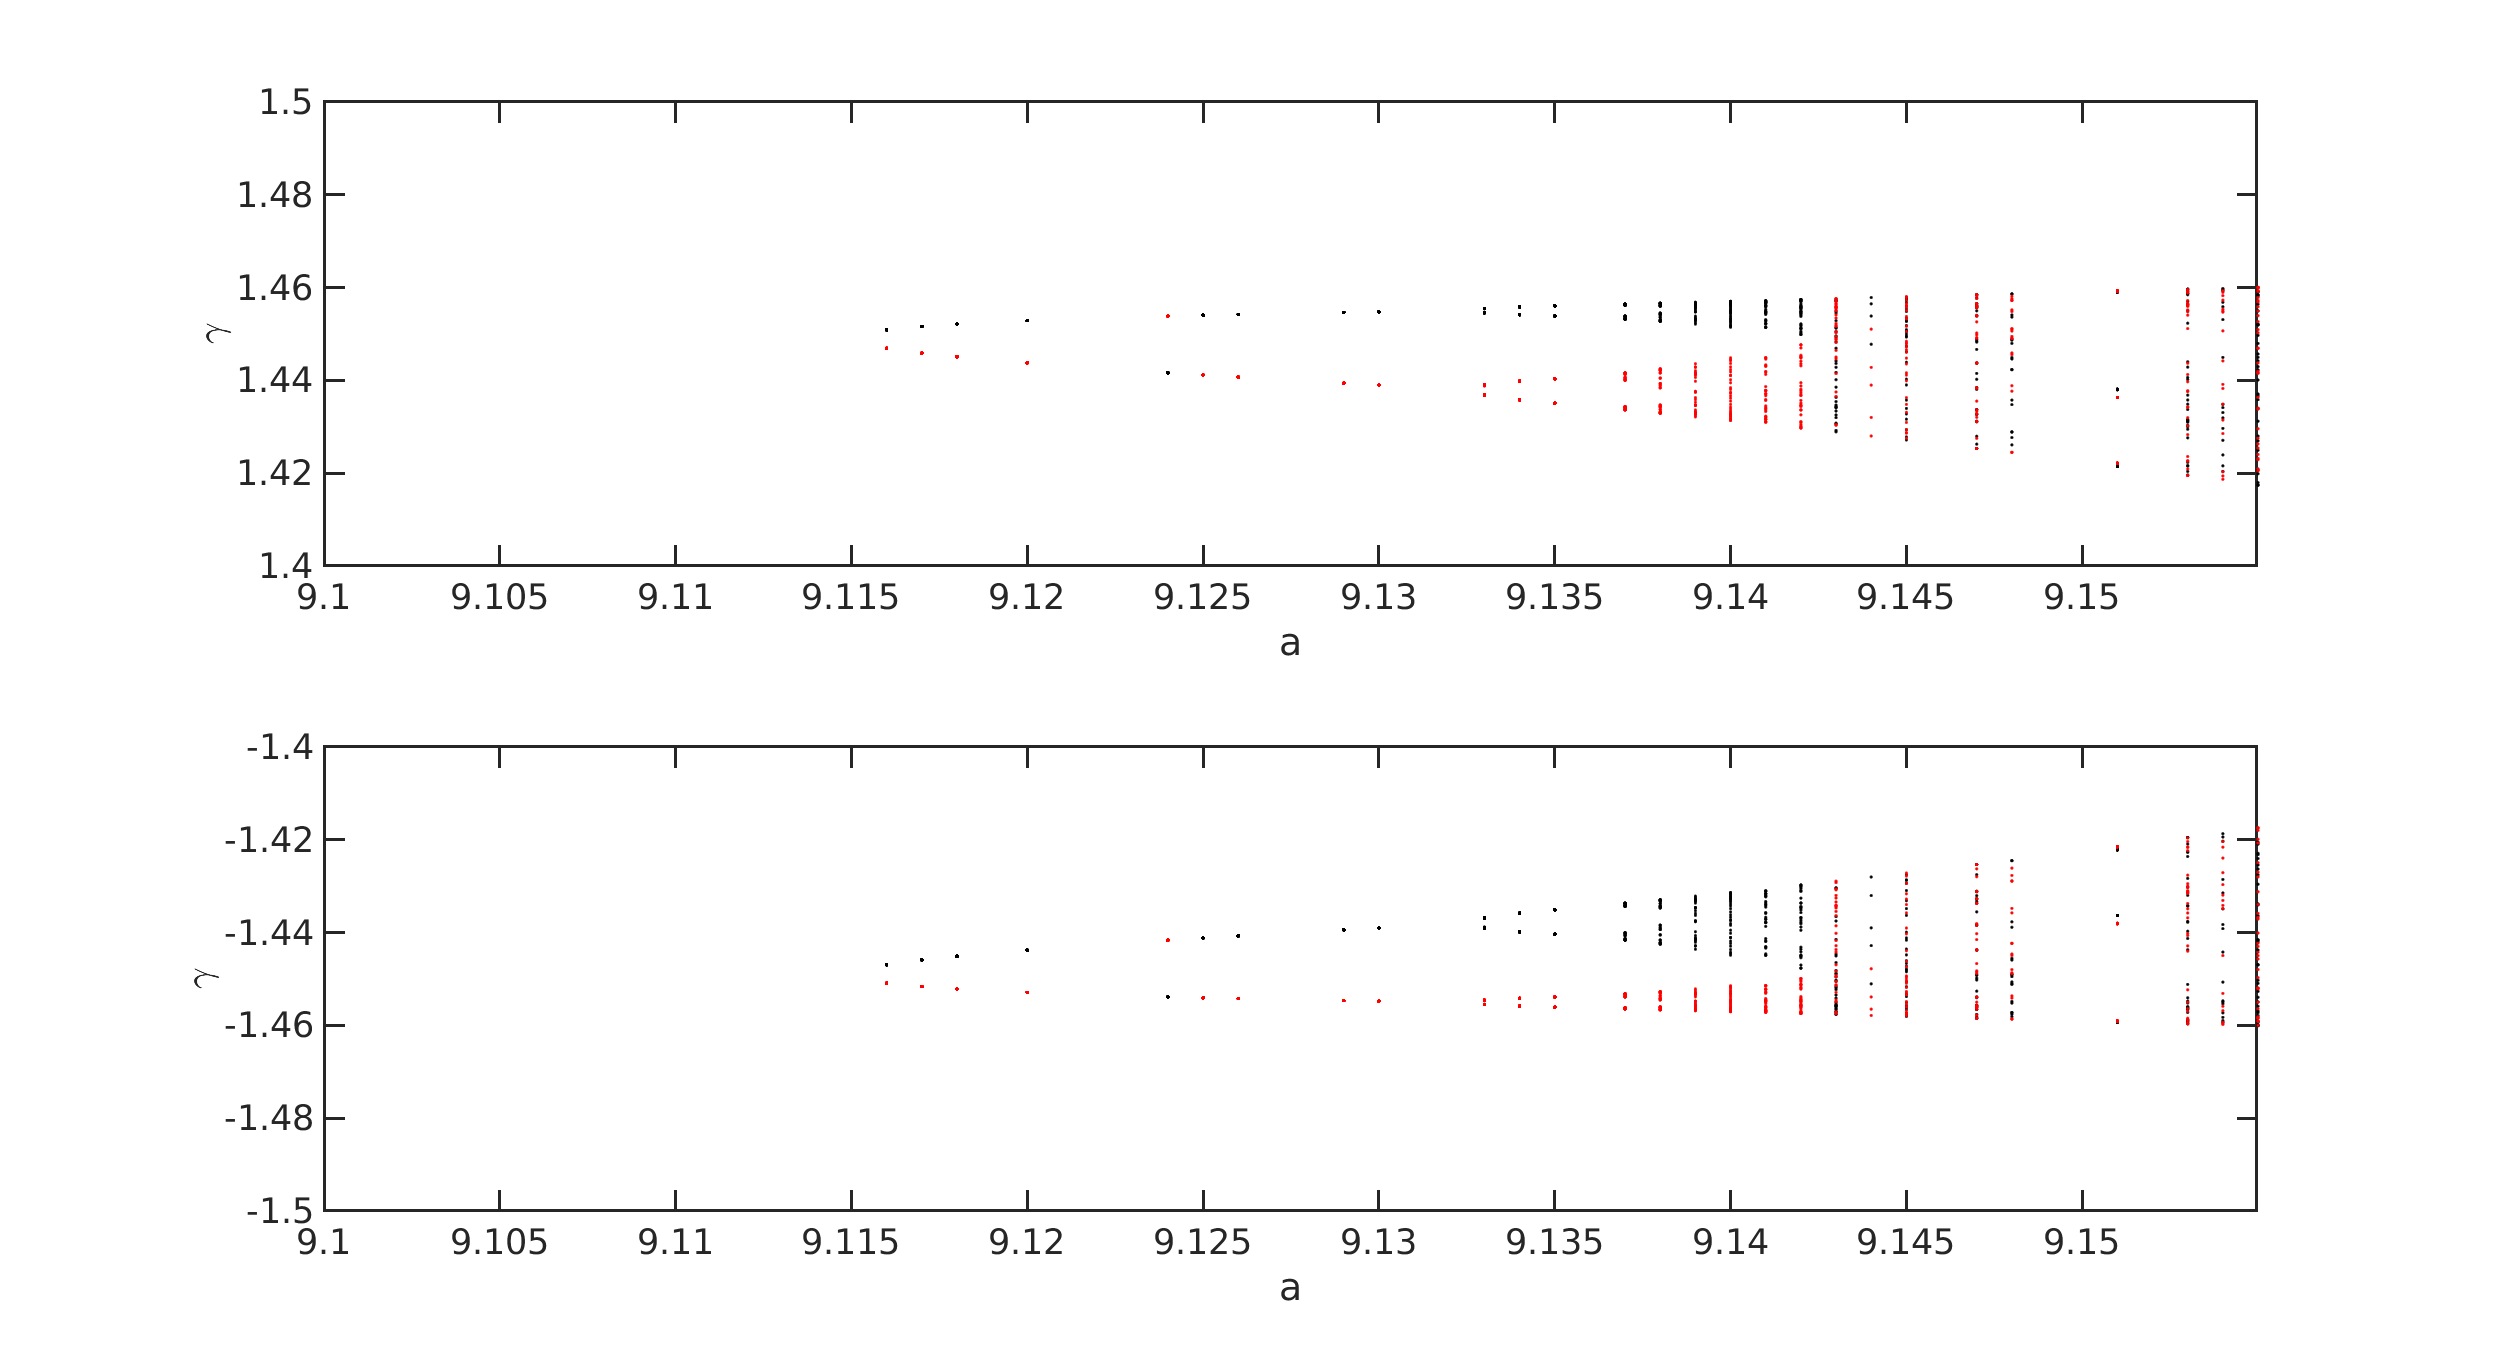
\includegraphics[width=\textwidth]{bifurcation_overlap2.png}
\caption{Bifurcation diagram with $\alpha = -\beta = -0.4$ and $\gamma_0 = \pm 1.45$.}
\label{fig:overlap2}
\end{figure}

\subsection{Robin transmission conditions}

We may change to Robin transmission conditions and find the same period doubling bifurcation pattern, albeit on a smaller scale.
Replace the Dirichlet transmission conditions ($u_1(\beta) = \gamma_n$, $u_2(\alpha) = u_1(\alpha)$) with the optimal Robin transmission conditions ($u_1'(\beta) + p u_1(\beta) = \gamma_n$, $u_2'(\alpha) - p u_2(\alpha) = u_1'(\alpha) - p u_1'(\alpha)$).
The bifurcation for $p=1$ and $\alpha = -\beta = -0.2$ may be seen in figure \ref{fig:Robin}.
The initial guesses are $\gamma_0 = \pm 3.1$.

\begin{figure}
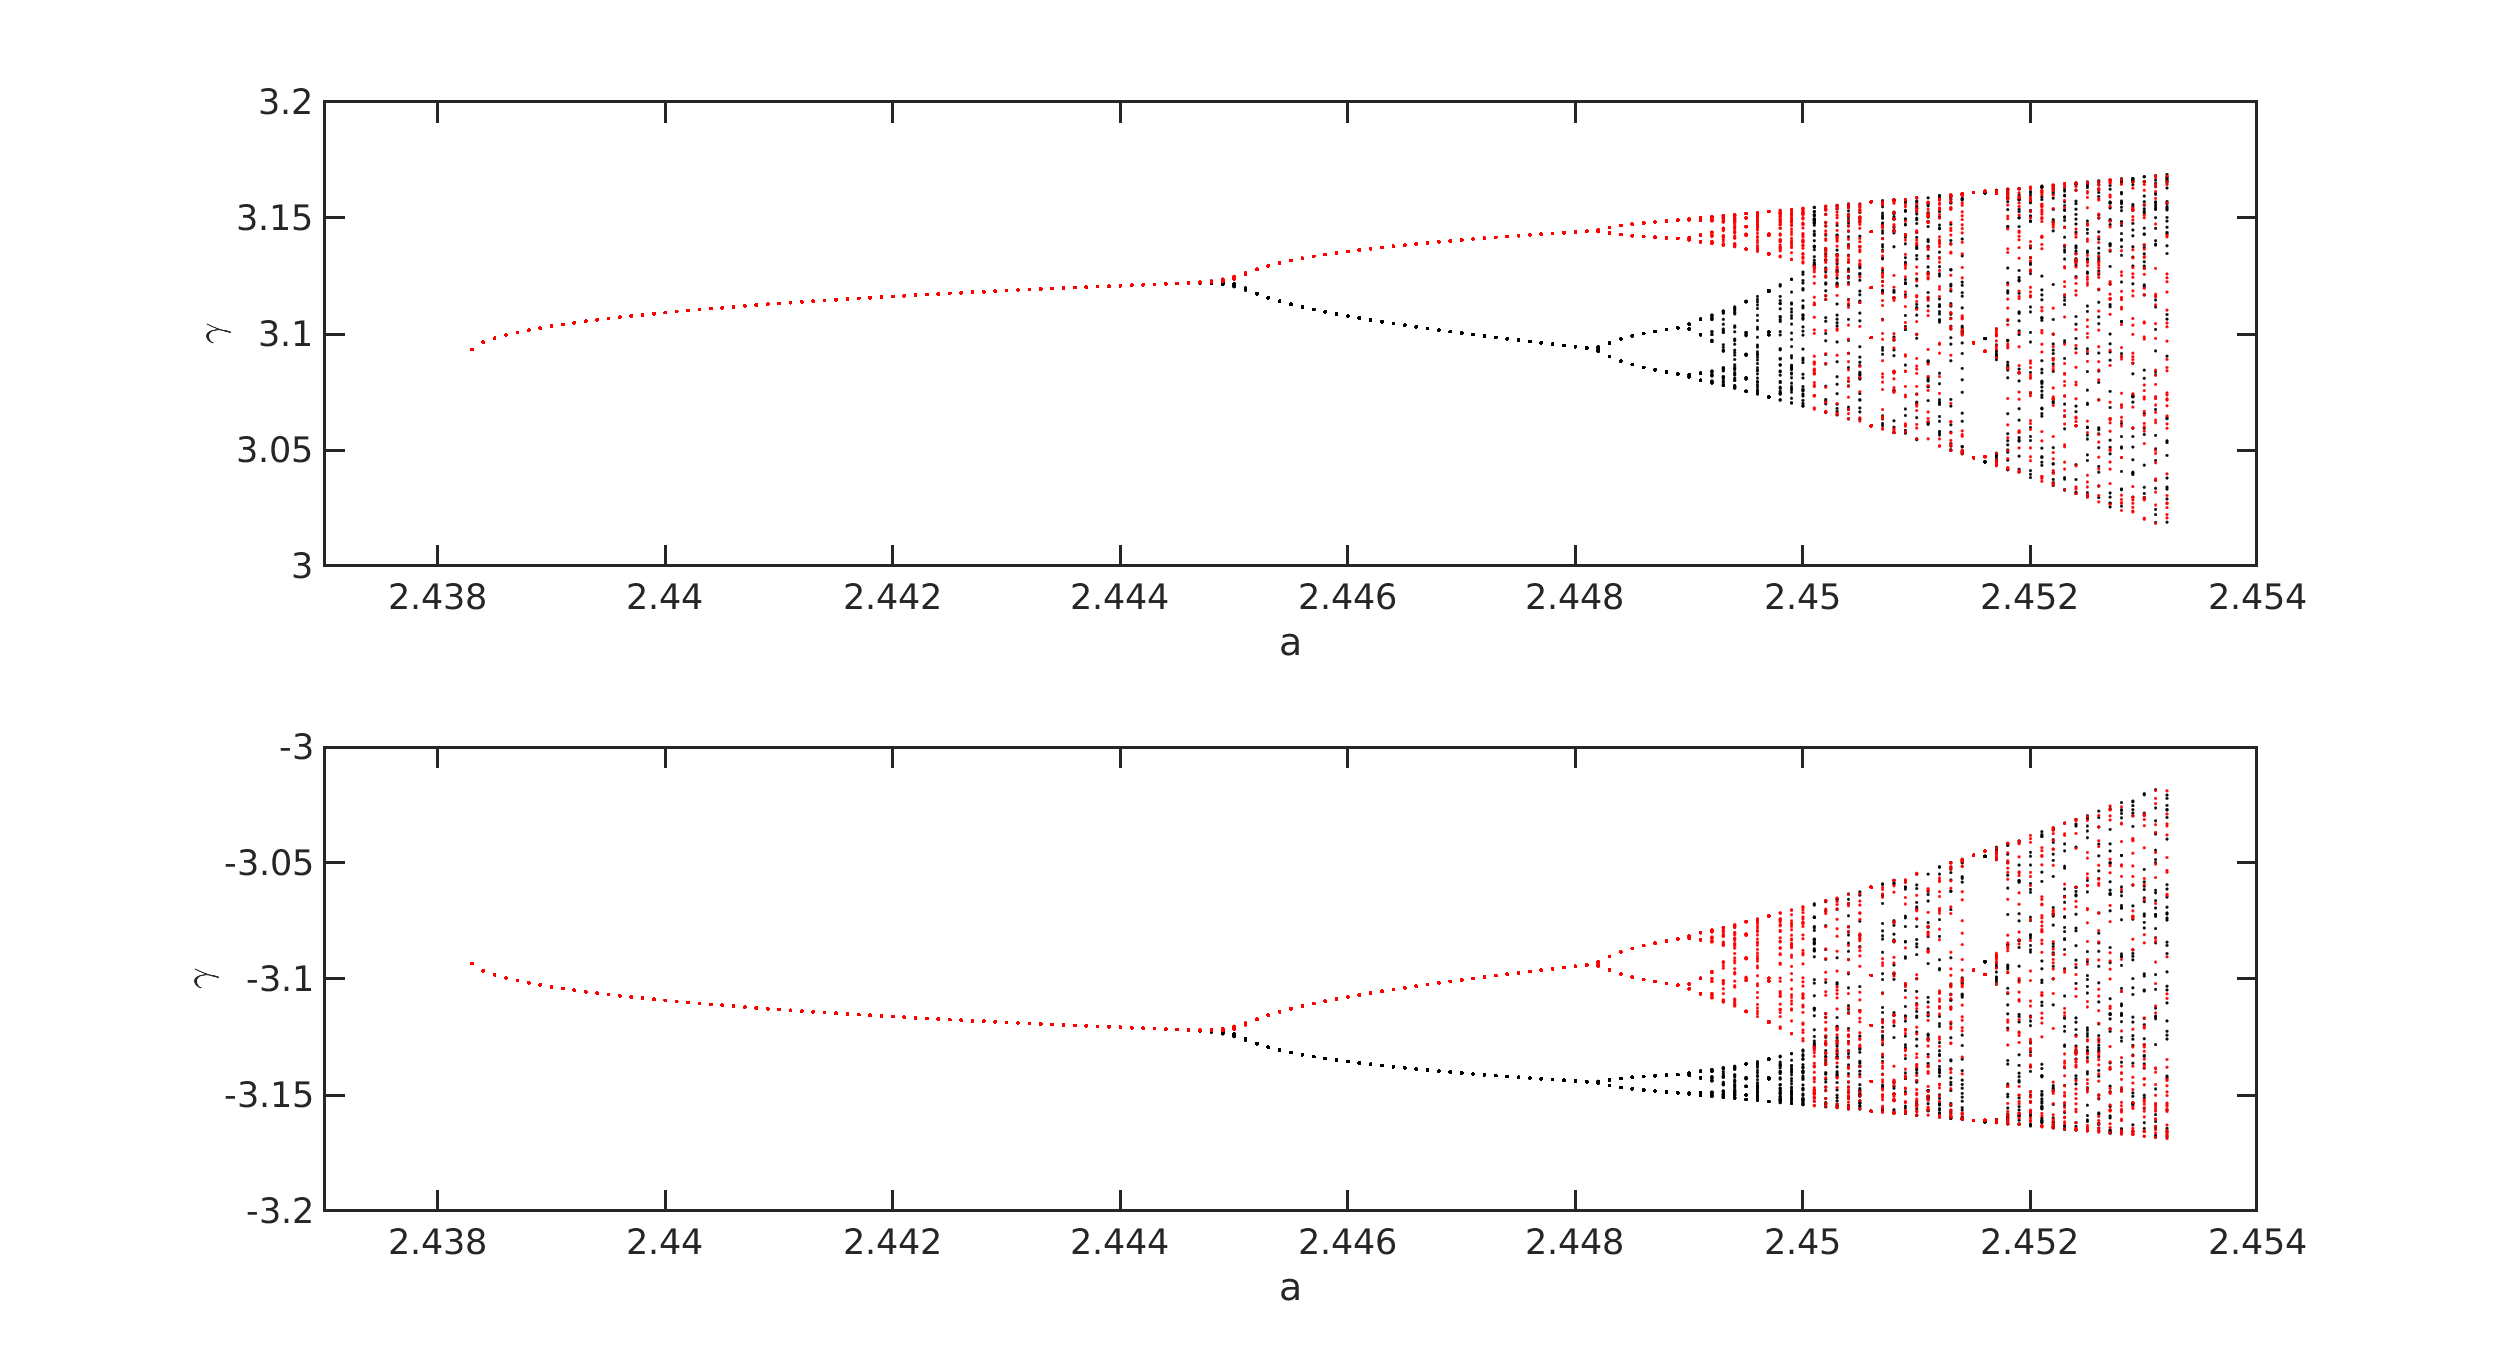
\includegraphics[width=\textwidth]{bifurcation_Robin.png}
\caption{Bifurcation diagram using Robin transmission conditions with $p=1$, $\alpha = -\beta = -0.2$ and $\gamma_0 = \pm 3.1$.}
\label{fig:Robin}
\end{figure}

\subsection{2D version}

We set up the following problem in 2D:
\begin{equation*}
\Delta u - \sin(au) = 0
\end{equation*}
on the square $[-1,1] \times [-1,1]$ with homogeneous Dirichlet boundary conditions on all sides.
The function $G(\gamma)$ is now a function acting on the space of functions over $[-1,1]$ and returns an element of the same.
In the discrete version, $G(\gamma)$ takes a vector and returns a vector of the same size.
We are now concerned with where $\norm{G(\gamma) - \gamma^*} \leq \norm{\gamma - \gamma^*}$.

A cursory search for values of $a$ that will produce cycles results in figure \ref{fig:Lap1} with $a = 33.8$.
Note that the initial guess is now a function, and we use $\gamma_0 = \tilde{\gamma}_0 (1 - x^2)$.
As it is impossible to present the fixed point function as the high dimensional object it is, figure \ref{fig:Lap1} shows the norm of $N(\gamma)$ as a function of $\tilde{\gamma}_0$.

There are clearly regions where $N(\gamma)$ is farther from the fixed point than $\gamma$.
However, tests of these regions show that the iterations there do not result in period doubling but instead are a random mixture of divergent, convergent and chaotic behaviour.
For example, $a = 33.755$ has a chaotic behaviour when $\tilde{\gamma}_0 = 1.8$, but a perturbation on the order of machine epsilon to this value of $a$ has convergent behaviour.

\begin{figure}
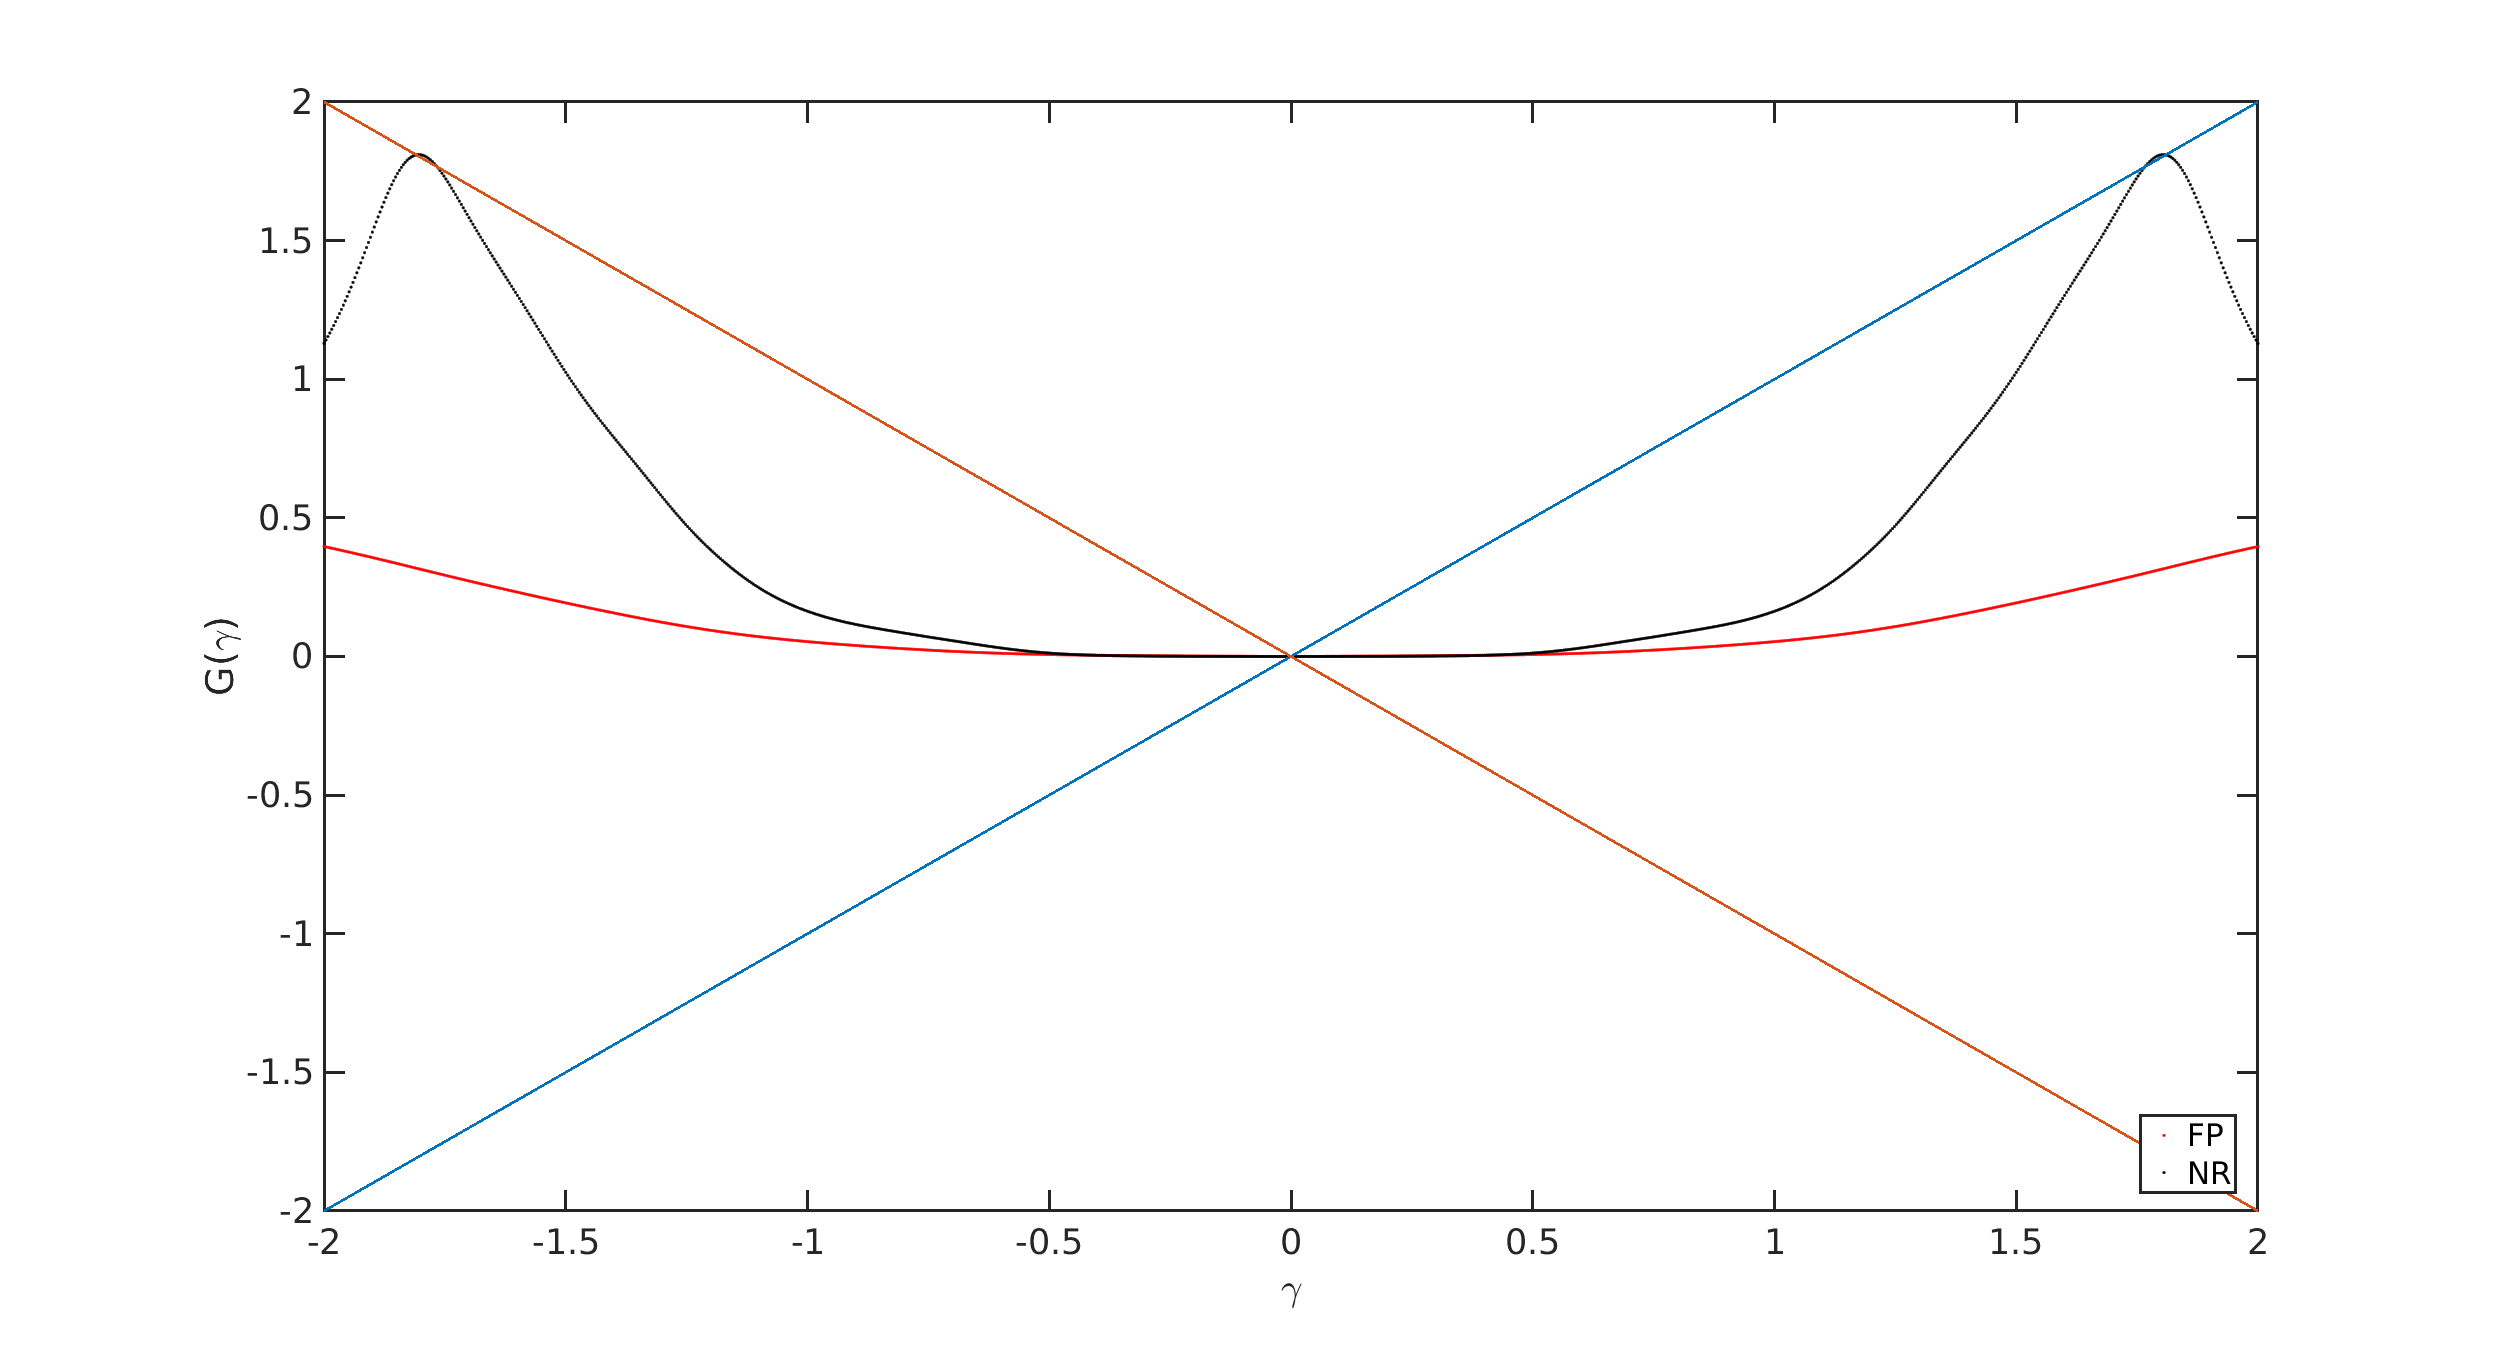
\includegraphics[width=\textwidth]{exp16_01.png}
\caption{The norm of $G(\gamma)$ and $N(\gamma)$ using $\gamma_0 = \tilde{\gamma}_0 (1 - x^2)$, plotted against the norm of $\gamma_0$.}
\label{fig:Lap1}
\end{figure}

We remove the $y$--derivatives from the equation and repeat the experiments.
The search for values of $a$ yields figure \ref{fig:2Dsearch}.
For this figure $\alpha = -\beta = -0.2$ and there are 21 points in both the $x$-- and $y$--directions.

\begin{figure}
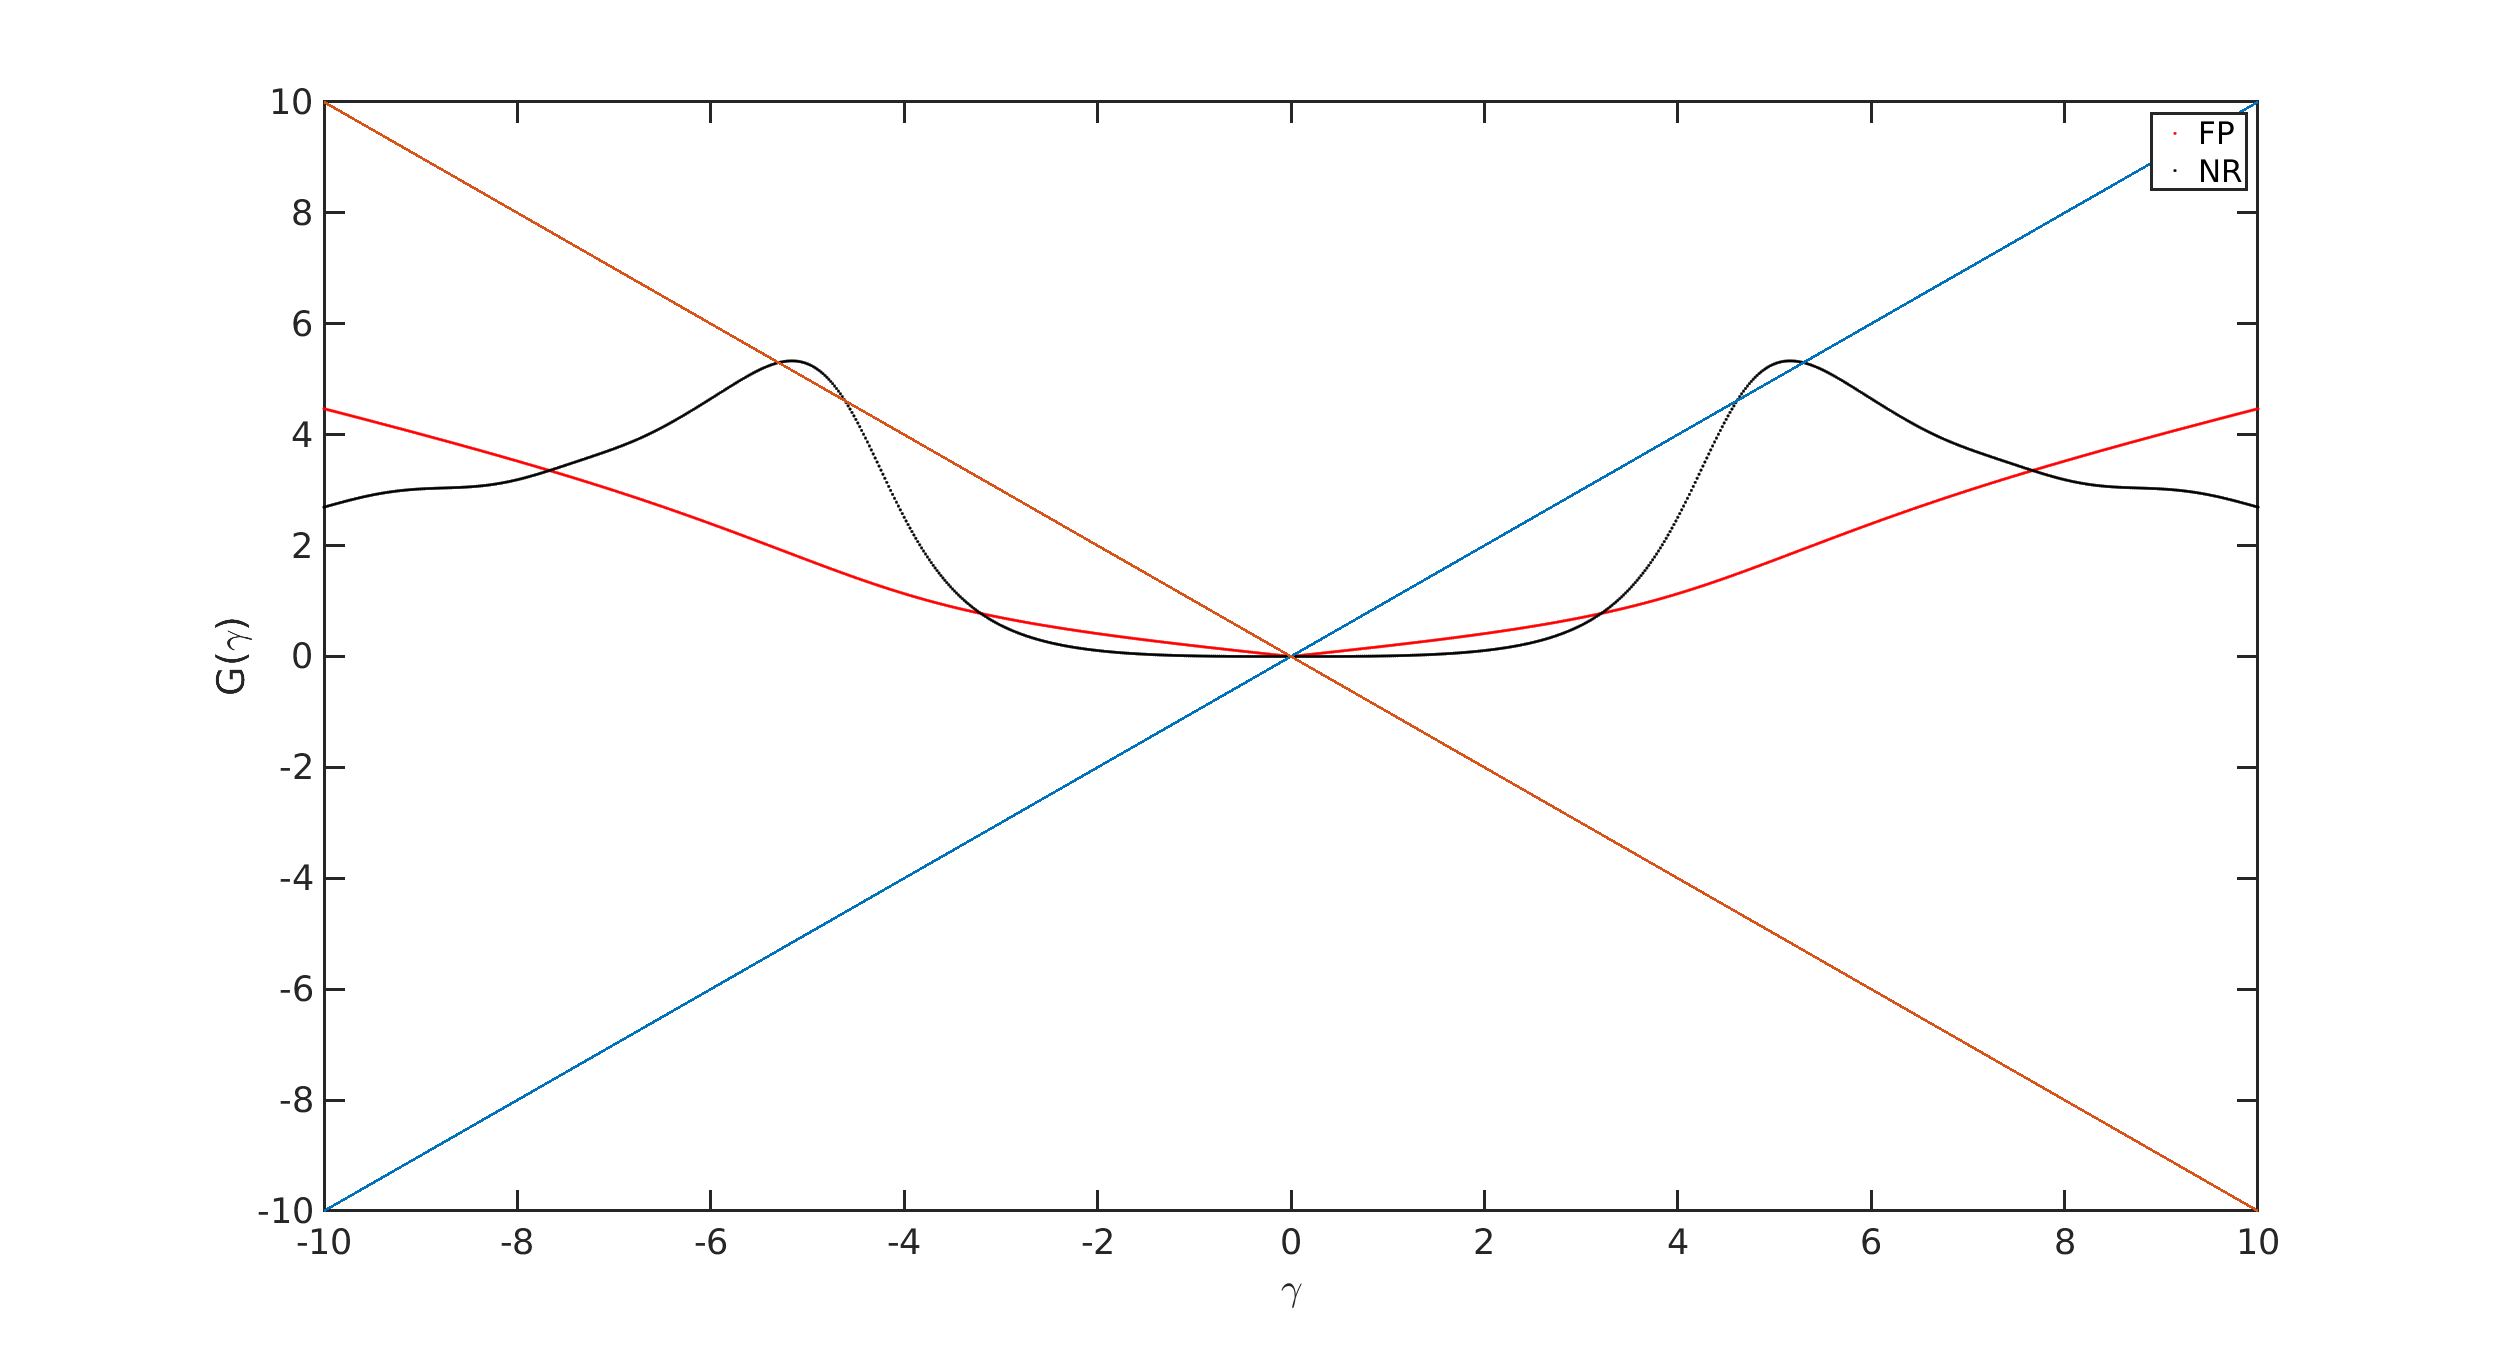
\includegraphics[width=\textwidth]{exp16_02.png}
\caption{}
\label{fig:2Dsearch}
\end{figure}

Using $\gamma_0 = \pm 8 (1-x^2) / \norm{1 - x^2}$ we find the bifurcation diagram shown in figure \ref{fig:2Dbifurc}.
Note also that $\alpha = -\beta = -0.2$ and there are 51 points in both the $x$-- and $y$--directions.
The number of points affects the requisite $\gamma_0$ for bifurcation but not its overall shape, it appears.
We note that the interval of bifurcation is roughly the same as that for the 1D case, suggesting a connection.

\begin{figure}
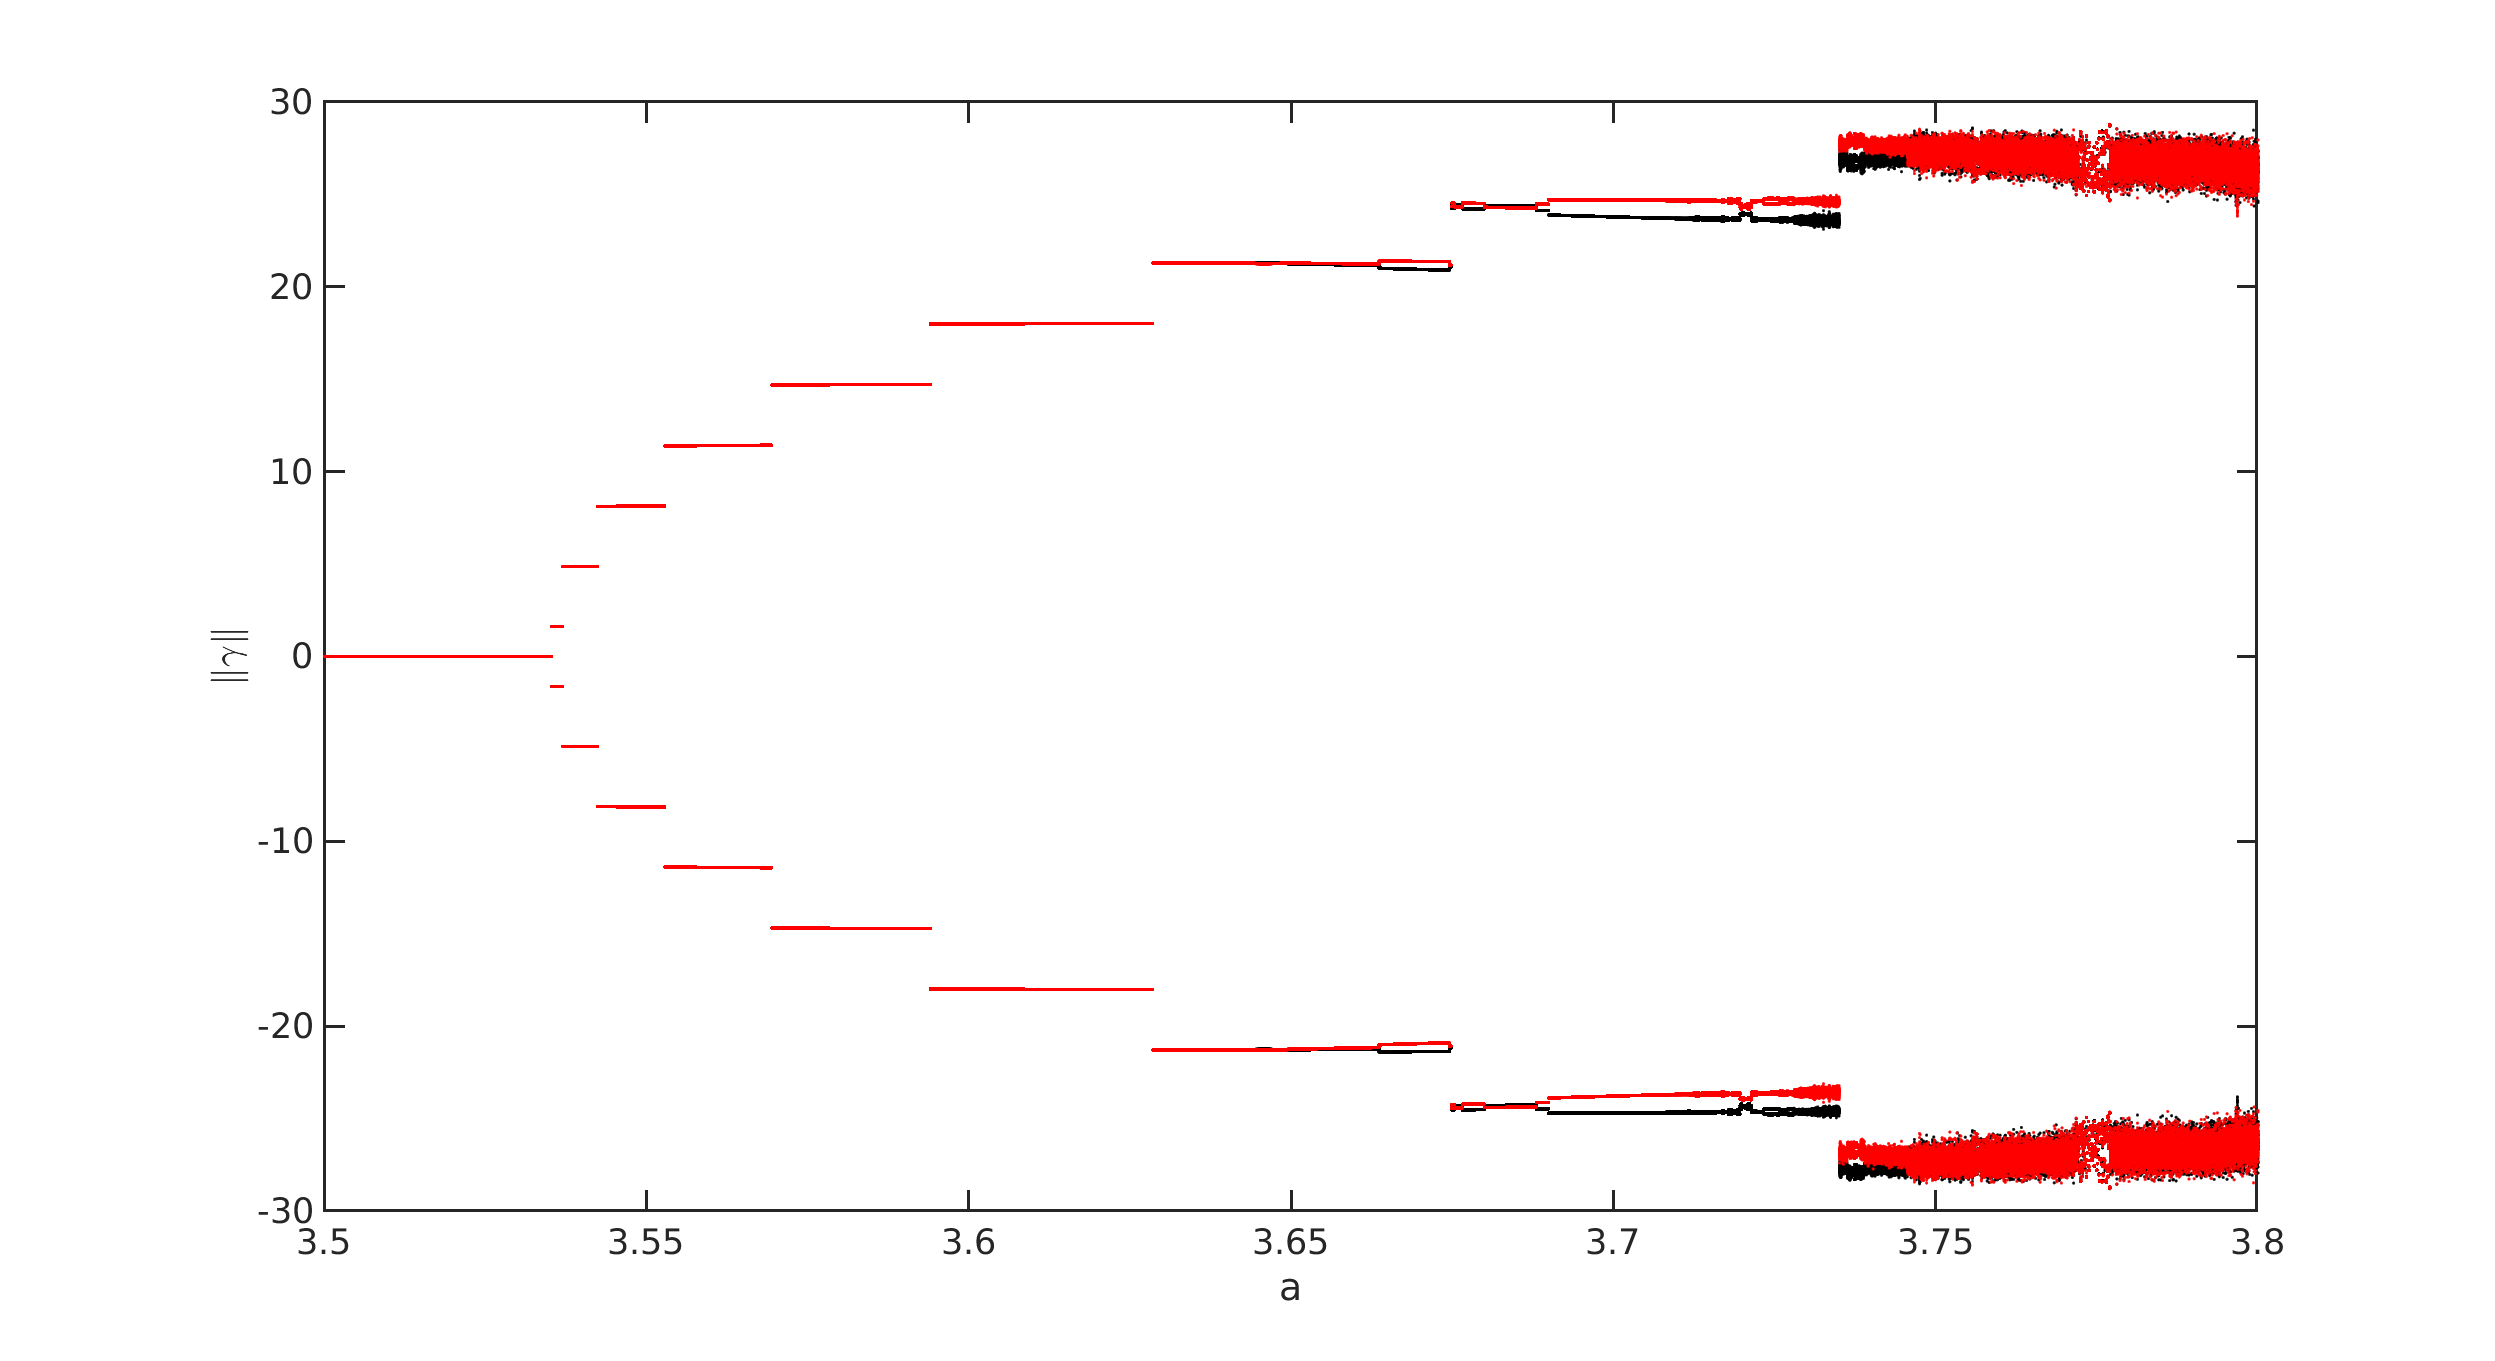
\includegraphics[width=\textwidth]{exp15_02.png}
\caption{}
\label{fig:2Dbifurc}
\end{figure}

\section{Proposed algorithm}
\label{sec:algo}

We have seen in the previous section that we cannot guarantee the monotonicity of $C(\gamma)$, nor the region of $G(\gamma)$ with general transmission conditions.
However, we have also shown that under certain assumptions we can ensure $G(\gamma)$ lies within region 2.
With this in mind, one may construct an algorithm to take advantage of the many properties discussed.
This incorporates Branin's corrections to the Newton-Raphson method as well as checks on various conditions on $G$ and $G'$.

\subsection{Notation and assumptions}

Steps (1) through (3) from equation (\ref{alg:ASPN}) remain unchanged.
We will replace step (4) with (4*), and step (5) by
\begin{equation*}
(5*) \quad \tilde{\gamma}_n = \gamma_n - \frac{u_2(\beta) - \gamma_n}{\abs{g_1(\alpha) g_3(\beta) - 1}} .
\end{equation*}
All affiliated functions and variables, including $F$, $J$ and $G(\gamma)$, are as described in section \ref{sec:appl}.

Regions 1 through 4 are defined in section \ref{sec:fpi}.
The function $C(\gamma)$ is defined in section \ref{sec:appl} but explained in greater detail in sections \ref{sec:nrm} and \ref{sec:nrfp}.
The corresponding lines $g_C(\gamma)$ may be found in section \ref{sec:nrfp}.

It is assumed that $G(\gamma)$ lies within region 2.
See theorem \ref{thm:lui} for an example of conditions that will guarantee this.

\subsection{Algorithm steps}

\begin{description}
\item[1.] Select some $\gamma_0 \in \mathbb{R}$. Set $n=0$.
\item[2.] Calculate $G(\gamma_n)$ using steps (1) and (2) from equation (\ref{alg:ASPN}) and $G'(\gamma_n)$ using steps (3) and (4*).
If $G'(\gamma_n) = 1$ then set $\gamma_{n+1} = G(\gamma_n)$, increment $n$ and return to step 2.
If this is not true, proceed to step 3.
\item[3.] Perform step (5*).
If $\abs{G'(\gamma_n) - 1} \geq 1/2$ then set $\gamma_{n+1} = \tilde{\gamma}_n$, increment $n$ and return to step 2.
If this is not true, calculate $\hat{\gamma}_n$, the average of $\gamma_n$ and $\tilde{\gamma}_n$, and proceed to step 4.
\item[4.] Use steps (1) and (2) to calculate $G(\hat{\gamma}_n)$.
If $G(\hat{\gamma}_n)-\hat{\gamma}_n$ has the same sign as $G(\gamma_n) - \gamma_n$ then set $\gamma_{n+1} = \tilde{\gamma}_n$, increment $n$ and return to step 2.
If this is not true, set $\gamma_{n+1} = G(\gamma_n)$, increment $n$ and return to step 2.
\end{description}

\subsection{Explanation of the algorithm}

In step 2 of the algorithm, we use fixed point iteration if $G'(\gamma_n) = 1$.
The Newton-Raphson iteration, even with Branin's adjustment, will calculate an infinite result if we proceed to step 3.
Since $G(\gamma)$ lies within region 2 we are certain that a fixed point step will always converge, however slowly.
Therefore, one may avoid the problem by using the slower method.

In steps 3 and 4, we use the calculated Newton-Raphson iteration only if we guarantee such an iteration lies within regions 2 and 3.
As has been shown in section \ref{sec:nrfp}, if $G'(\gamma) < 1/2$ then the iteration is certainly within regions 2 and 3.
By using Branin's adjustment, we also have this fact for $G'(\gamma) > 3/2$.

Step 4 checks if the Newton-Raphson iteration lies within region 4.
Since we know the geometry along which the boundary of regions 3 and 4 is defined, we can calculate the following scenario:
we suppose that the point $(\gamma_n, G(\gamma_n))$ lies on this boundary.
The line $g_C(\gamma)$ at this point intersects the line $y=x$ at the point $\hat{\gamma}_n$.
If the fixed point lies between $\gamma_n$ and $\hat{\gamma}_n$ then the point lies within region 4.

To check which side of $\hat{\gamma}_n$ the fixed point lies, we need to test $G(\hat{\gamma}_n)$.
If $G(\hat{\gamma}_n) - \hat{\gamma}_n$ has the same sign as $G(\gamma_n) - \gamma_n$ then both $\hat{\gamma}_n$ and $\gamma_n$ lie on the same side of the fixed point, and the iteration lies in regions 2 and 3.
If not, they lie on different sides of the fixed point and so the fixed point must lie between them.
In this instance, the iteration lies in region 4 and to avoid spiralling away from the fixed point one should use the fixed point iteration which, as has already been stated, is guaranteed to converge.

In this way, all possibilities are accounted for: region 1 cannot occur due to Branin's adjustment and the avoidance of $G'(\gamma_n) = 1$; region 4 is tested for extensively and whenever it occurs the algorithm uses a method that is guaranteed to converge under the assumptions listed previously.

\bibliographystyle{plain}
\bibliography{C:/Users/conmc/Documents/LaTeX/references}

\end{document}